\documentclass[
	12pt,				% tamanho da fonte
	openany,			% capítulos começam em pág ímpar (insere página vazia caso preciso)
	oneside, 			% oneside - twoside
	a4paper,			% tamanho do papel.
	chapter=TITLE,		% títulos de capítulos convertidos em letras maiúsculas
	section=TITLE,		% títulos de seções convertidos em letras maiúsculas
	sumario=tradicional,	
	%subsection=TITLE,	% títulos de subseções convertidos em letras maiúsculas
	%subsubsection=TITLE,% títulos de subsubseções convertidos em letras maiúsculas
	english,			% idioma adicional para hifenização
	brazil,				% o último idioma é o principal do documento
	]{abntex2}

% ---------------------------------------------------------------------------
% Inclui os comandos do projeto
% ---------------------------------------------------------------------------
% -----------------------------------------------------------------------------
% Pacotes fundamentais
% -----------------------------------------------------------------------------
\usepackage{xcolor}
\newcommand\myworries[1]{\textcolor{red}{[#1]}}
\usepackage{lmodern}		% Usa a fonte Latin Modern (Serifada, tipo Times New Roman
%\usepackage{helvet}		% Usa a fonte Helvetica (Tipo Arial)	
%\renewcommand{\familydefault}{\sfdefault} tira o serifado
\usepackage[T1]{fontenc}		% Selecao de codigos de fonte.
\usepackage[utf8]{inputenc}		% Codificacao do documento (conversão automática dos acentos)
\usepackage{indentfirst}		% Indenta o primeiro parágrafo de cada seção.
\usepackage{color}				% Controle das cores
\usepackage{tikz}				% Inclusão de gráficos
\usepackage{graphicx}			% Inclusão de gráficos
\usepackage{microtype} 			% para melhorias de justificação
% -----------------------------------------------------------------------------
% Pacotes adicionais, usados no anexo do modelo de folha de identificação
% -----------------------------------------------------------------------------
\usepackage{multicol}
\usepackage{multirow}
% -----------------------------------------------------------------------------
% Pacotes adicionais, usados apenas no âmbito do Modelo Canônico do abnteX2
% -----------------------------------------------------------------------------
\usepackage{lipsum}				% para geração de dummy text
% -----------------------------------------------------------------------------
% Pacotes de citações
% -----------------------------------------------------------------------------
\usepackage[brazilian,hyperpageref]{backref}	 % Paginas com as citações na bibliografia
\usepackage[alf,abnt-etal-list=3,abnt-etal-cite=3, abnt-emphasize=bf]{abntex2cite}	% Citações padrão ABNT
\usepackage{pdflscape}
\usepackage{footnote}
\usepackage{pdfpages}
\usepackage{caption}

% -----------------------------------------------------------------------------
% Pacotes adicionados por @leolleocomp
% ----------------------------------------------------------------------------- 
\usepackage{booktabs}
\usepackage{adjustbox}
\usepackage{subcaption}
\usepackage[labelfont=bf]{caption}
\usepackage{gensymb}
\usepackage{amsmath}
\usepackage{array}
\usepackage{float}
\usepackage{xcolor,colortbl}
\usepackage{longtable}
\usepackage{scalefnt}
\usepackage{listings}			% inserir codigo fonte


% -----------------------------------------------------------------------------
% Pacotes adicionados por @Gabrielr2508
% ----------------------------------------------------------------------------- 
\usepackage{hyperref}

\usepackage{tocloft}
% -- permite a adição de células especiais em tabelas
\newcommand{\specialcell}[2][c]{%
  \begin{tabular}[#1]{@{}c@{}}#2\end{tabular}}

\newcounter{equationset}
\newcommand{\equationset}[1]{% \equationset{<caption>}
  \refstepcounter{equationset}% Step counter
  \noindent\makebox[\linewidth]{Equação ~\theequationset: #1}
 }

%--------------------------------------------------------------------------------
% Adequação dos títulos dos capitulos, seções, subseções às normas da Univasf
% Added by @Gabrielr2508
%--------------------------------------------------------------------------------
\renewcommand{\ABNTEXchapterfont}{\fontseries{b}}
\renewcommand{\ABNTEXchapterfontsize}{\normalsize}

\renewcommand{\ABNTEXsectionfont}{\fontseries{m}}
\renewcommand{\ABNTEXsectionfontsize}{\normalsize}

\renewcommand{\ABNTEXsubsectionfont}{\fontseries{b}}
\renewcommand{\ABNTEXsubsectionfontsize}{\normalsize}

\renewcommand{\ABNTEXsubsubsectionfont}{\fontseries{m}}
\renewcommand{\ABNTEXsubsubsectionfontsize}{\normalsize}

%--------------------------------------------------------------------------------
% CONFIGURAÇÕES DE PACOTES
% Configurações do pacote backref
%--------------------------------------------------------------------------------
% Usado sem a opção hyperpageref de backref
\renewcommand{\backrefpagesname}{Citado na(s) página(s):~}
% Texto padrão antes do número das páginas
\renewcommand{\backref}{}
% Define os textos da citação
\renewcommand*{\backrefalt}[4]{
	\ifcase #1 %
		%Nenhuma citação no texto.%
	\or
		Citado na página #2.%
	\else
		Citado #1 vezes nas páginas #2.%
	\fi}%

%--------------------------------------------------------------------------------
% Configurações de aparência do PDF final
%--------------------------------------------------------------------------------
% alterando o aspecto da cor azul
\definecolor{blue}{RGB}{41,5,195}

% informações do PDF
\makeatletter
\hypersetup{
     	%pagebackref=true,
		pdftitle={\@title},
		pdfauthor={\@author},
    	pdfsubject={\imprimirpreambulo},
	    pdfcreator={LaTeX with abnTeX2},
		pdfkeywords={abnt}{latex}{abntex}{abntex2}{relatório técnico},
		colorlinks=true,			% false: boxed links; true: colored links
    	linkcolor=black,				% color of internal links
    	citecolor=black,				% color of links to bibliography
    	filecolor=black,			% color of file links
		urlcolor=black,
		bookmarksdepth=4
}
\makeatother
% ---

% ---
% Espaçamentos entre linhas e parágrafos
% ---

% O tamanho do parágrafo é dado por:
\setlength{\parindent}{1.3cm}

% Controle do espaçamento entre um parágrafo e outro:
\setlength{\parskip}{0.2cm}  % tente também \onelineskip

%--------------------------------------------------------------------------------
% compila o indice
%--------------------------------------------------------------------------------
\makeindex
% ---

%--------------------------------------------------------------------------------
% Comando para inserir imagens de forma simples
%--------------------------------------------------------------------------------
\newcommand{\imagem}[4]
{%			\imagem{x.x}{nomeimg}{titulo}{fonte}
	\begin{figure}[!htb]
		\caption{\label{img:#2}#3}
		\begin{center}
			\includegraphics[scale=#1]{img/#2}
		\end{center}
        \legend{\textbf{Fonte:} #4}
	\end{figure}
}%

%--------------------------------------------------------------------------------
% Creio que esses comandos sejam para desenhar algo, aguardando explicações de @leolleocomp
%--------------------------------------------------------------------------------
\newcommand{\xx} {$\bigotimes$}
\newcommand{\oo} {$\bigcirc$}

%--------------------------------------------------------------------------------
% Biblioteca para códigos-fonte
%--------------------------------------------------------------------------------
\usepackage[newfloat=true]{minted}

%--------------------------------------------------------------------------------
% Caixas batutas - by @leolleocomp
%--------------------------------------------------------------------------------
\usepackage[most]{tcolorbox}
\tcbuselibrary{breakable}

\tcbuselibrary{minted}
\tcbset{listing engine=minted}

\definecolor{bg}{rgb}{0.95,0.95,0.95}

\SetupFloatingEnvironment{listing}{name=Código, listname=Lista de códigos}

%--------------------------------------------------------------------------------
% configuração do contador dos códigos-fonte - by @leolleocomp
% assim como as figuras, começa em 1
\newcounter{sourcecode}
%--------------------------------------------------------------------------------
%--------------------------------------------------------------------------------
% @leolleocomp
% stackoverflow code
% peguei da resposta abaixo
% https://stackoverflow.com/questions/24086366/change-latex-minted-listings-numbering-to-include-current-section?answertab=votes#tab-top
%--------------------------------------------------------------------------------
\makeatletter
\renewcommand*{\thelisting}{\thesourcecode}
\makeatother

%--------------------------------------------------------------------------------
% Peçam explicações a @leolleo
% WHO DID THIS?
%--------------------------------------------------------------------------------
\newcommand{\Ididthis}{
%	\legend{\textbf{Fonte:} O autor (\the\year).}
\legend{\textbf{Fonte:} O autor}
}

\newcommand{\Otherguydidthis}[1]{
	\legend{\textbf{Fonte:} \citeonline{#1}.}
}

%--------------------------------------------------------------------------------
% Comando para inserir códigos - by @leolleocomp
%--------------------------------------------------------------------------------
\newcommand{\sourcecode}[4]{
\begin{listing}[H]
	\refstepcounter{sourcecode}
	\caption{#1}
	\label{cmd:#2}
	\inputminted[linenos, bgcolor=bg, tabsize=4,breaklines]{#3}{codes/#4}
	\Ididthis
\end{listing}
}

% -----------------------------------------------------------------------------
% Pacotes adicionados por @ruanmed
% ----------------------------------------------------------------------------- 
\usepackage[binary-units=true]{siunitx}


%--------------------------------------------------------------------------------
% Comando para inserir códigos - by @ruanmed
%--------------------------------------------------------------------------------
\newcommand{\Wedidthis}{%   \legend{\textbf{Fonte:} O autor (\the\year).}
    \legend{\textbf{Fonte:} Os autores.}
}
 
%--------------------------------------------------------------------------------
% Comando para inserir códigos - by @ruanmed
%--------------------------------------------------------------------------------
\usepackage{caption}
 
\newenvironment{code}{\captionsetup{type=listing}}{}
\SetupFloatingEnvironment{listing}{name=Código}
 
\newcommand{\sourcecodenolist}[4]{
    \begin{code}
        \refstepcounter{sourcecode}
       \caption[]{#1}
       \label{code:#2}
       \inputminted[linenos, bgcolor=bg, tabsize=4,breaklines]{#3}{codes/#4}
       \Wedidthis
   \end{code}
}

% \newcommand{\sourcecodenolist}[4]{
% 	\refstepcounter{sourcecode}
% 	\captionof{listing}{#1 \label{cmd:#2}}
% 	\inputminted[linenos, bgcolor=bg, tabsize=4,breaklines]{#3}{codes/#4}
% 	\Wedidthis
% }

% \newcommand{\sourcecodenolist}[4]{
% 	\refstepcounter{sourcecode}
% 	\captionof{listing}{#1 \label{cmd:#2}}
% 	\inputminted[linenos, bgcolor=bg, tabsize=4,breaklines]{#3}{codes/#4}
% 	\Wedidthis
% }


\newcommand{\sourcecodeinline}[2]{
	\mintinline[linenos, bgcolor=bg, tabsize=4,breaklines]{#1}{#2}
}
% CONFIGURACAO DO SUMARIO
%-------------------------------------------------------------------------------
% Modifica o espaçamento no sumário
% Nao ha espacos, exceto para as entradas de capitulos
\setlength{\cftbeforeparagraphskip}{0pt}
\setlength{\cftbeforesubsectionskip}{0pt}
\setlength{\cftbeforesectionskip}{0pt}
\setlength{\cftbeforesubsubsectionskip}{0pt}
\setlength{\cftbeforechapterskip}{\onelineskip}

% Alteração da indentação dos itens do sumário
\cftsetindents{chapter}{0pt}{42pt}
\cftsetindents{section}{0pt}{42pt}
\cftsetindents{subsection}{0pt}{42pt}
\cftsetindents{subsubsection}{0pt}{42pt}

% Modifica a formatacao dos textos

% Secao Primaria (Chapter): Caixa alta, Negrito, tamanho 12
\makeatletter
\settocpreprocessor{chapter}{%
  \let\tempf@rtoc\f@rtoc%
  \def\f@rtoc{%
  \texorpdfstring{\bfseries\MakeTextUppercase{\tempf@rtoc}}{\tempf@rtoc}}%
}
\makeatother

\makeatletter
\newcommand{\customlabel}[2]{%
   \protected@write \@auxout {}{\string \newlabel {#1}{{#2}{\thepage}{#2}{#1}{}} }%
   \hypertarget{#1}{#2}
}
\makeatother

% ---------------------------------------------------------------------------
% IDENTIFICAÇÃO
% ---------------------------------------------------------------------------
\titulo{INVESTIGAÇÃO SOBRE UTILIZAÇÃO DE APRENDIZAGEM POR REFORÇO PARA MÓDULO DE DEFESA APLICADO AO FUTVASF2D}
\autor{JOÃO PEDRO FIGUEIRÔA NASCIMENTO}
\local{JUAZEIRO - BA}
\orientador{Prof. Dr. Rosalvo Ferreira de Oliveira}
%\coorientador{M. Sc. Osvaldo Campelo de Mello Vasconselos}
\instituicao{UNIVERSIDADE FEDERAL DO VALE DO SÃO FRANCISCO
	\par
CURSO DE GRADUAÇÃO EM ENGENHARIA DE COMPUTAÇÃO}
\tipotrabalho{Trabalho de Conclusão de Curso}
\preambulo{Trabalho apresentado à Universidade Federal do Vale do São Francisco - Univasf, Campus Juazeiro, como requisito da obtenção do título de Bacharel em Engenharia de Computação.}


% -----------------------------------------------------------------------------
% CONFIGURACAO DO SUMARIO - by @Gabrielr2508
% Precisa estar aqui, por isso não foi para o commands.tex, não descobrimos o motivo, %caso saiba, por favor, faça um pull request! :D
% -----------------------------------------------------------------------------
% Secao primaria (Chapter) Caixa alta, Negrito, tamanho 12
\makeatletter
\renewcommand*{\l@chapter}[2]{%
  \l@chapapp{\uppercase{#1}}{#2}{\cftchaptername}}
\makeatother
% Secao secundaria (Section) Caixa baixa, Negrito, tamanho 12
\renewcommand{\cftsectionfont}{\uppercase} %ponha \rmfamily se quiser serifadas...

% Secao terciaria (Subsection) Caixa baixa, negrito, tamanho 12
\renewcommand{\cftsubsectionfont}{\bfseries}

% Secao quaternaria (Subsubsection) Caixa baixa, tamanho 12
\renewcommand{\cftsubsubsectionfont}{\normalfont}

% Seção quinaria (subsubsubsection) Caixa baixa, sem negrito, tamanho 12
\renewcommand{\cftparagraphfont}{\normalfont\itshape}

% -----------------------------------------------------------------------------
% Início do TCC 
% -----------------------------------------------------------------------------
\begin{document}

	\frenchspacing % Retira espaço extra obsoleto entre as frases.
	
	\pretextual
		%--------------------------------------------------------------------------------
% Constrói a capa com base na seção de identificação do main.tex
%--------------------------------------------------------------------------------
\begin{capa}
    \setlength{\belowcaptionskip}{0pt}
    \setlength{\abovecaptionskip}{0pt}
    \setlength{\intextsep}{-18pt}
        \begin{figure}[h]
    		\begin{center}
    		    
\includegraphics[scale=1.0]{img/LOGO_UNIVASF_big.pdf}
    		\end{center}
    	\end{figure}

        %
\includegraphics[scale=0.6]{img/univasf.jpg}
        \center
    	{\ABNTEXchapterfont\large\imprimirinstituicao}

    	\vspace*{2cm}
    	    {\imprimirautor}
    	\vspace*{2cm}
    %	\vfill
        \begin{center}
    		\ABNTEXchapterfont\bfseries\large\imprimirtitulo
        \end{center}
    	\vfill

    	\ABNTEXchapterfont\bfseries\large\imprimirlocal\\ 
    	\the\year

    	\vspace*{1cm}
\end{capa}
%--------------------------------------------------------------------------------
% Constrói a folha de rosto com base na seção de identificação do main.tex
%--------------------------------------------------------------------------------
\begin{folhaderosto}
\center
    	{\ABNTEXchapterfont\large\imprimirinstituicao}

		\vspace*{2cm}
    	    {\imprimirautor}
    	\vspace*{2cm}
		\vspace*{\fill}

		{\ABNTEXchapterfont\bfseries\large\imprimirtitulo}
		\vspace*{\fill}

		{\hspace{.45\textwidth}
		\begin{minipage}{.5\textwidth}
			\SingleSpacing
			\imprimirpreambulo \\ \\

			{\imprimirorientadorRotulo~\imprimirorientador\par}
			{\imprimircoorientadorRotulo~\imprimircoorientador\par}

		\end{minipage}%
		\vspace*{\fill}}%
		\vspace*{\fill}
			\ABNTEXchapterfont\bfseries\large\imprimirlocal\\ 
			\the\year
		\vspace*{1cm}
\end{folhaderosto}

%--------------------------------------------------------------------------------
% Constrói a ficha catalográfia com base na seção de identificação do main.tex
% Está comentado porque no final das contas a biblioteca do seu campus que gera a 
% numeração, você pode adicionar os numeros aqui, ou anexar o pdf gerado por eles
% ao documento.
%--------------------------------------------------------------------------------
%\begin{fichacatalografica}
%	\vspace*{\fill}					% Posição vertical
%	\hrule							% Linha horizontal
%	\begin{center}					% Minipage Centralizado
%	\begin{minipage}[c]{12.5cm}		% Largura
%
%	\imprimirautor
%
%	\hspace{0.5cm} \imprimirtitulo  / \imprimirautor. --
%	\imprimirlocal, \the\year-
%
%	\hspace{0.5cm} xx p. : il. (algumas color.) ; 30 cm.\\
%
%	\hspace{0.5cm} \imprimirorientadorRotulo~\imprimirorientador\\
%
%	\hspace{0.5cm}
%	\parbox[t]{\textwidth}{\imprimirtipotrabalho~--~\imprimirinstituicao,
%	\the\year.}\\
%
%	\hspace{0.5cm}
%		1. Palavra-chave1.
%		2. Palavra-chave2.
%		I. Orientador.
%		II. Universidade xxx.
%		III. Faculdade de xxx.
%		IV. Título\\
%
%	\hspace{8.75cm} CDU 02:141:005.7\\
%
%	\end{minipage}
%	\end{center}
%	\hrule
%\end{fichacatalografica}

%--------------------------------------------------------------------------------
% Anexando a ficha catalogáfica e a folha de aprovação 
%--------------------------------------------------------------------------------
%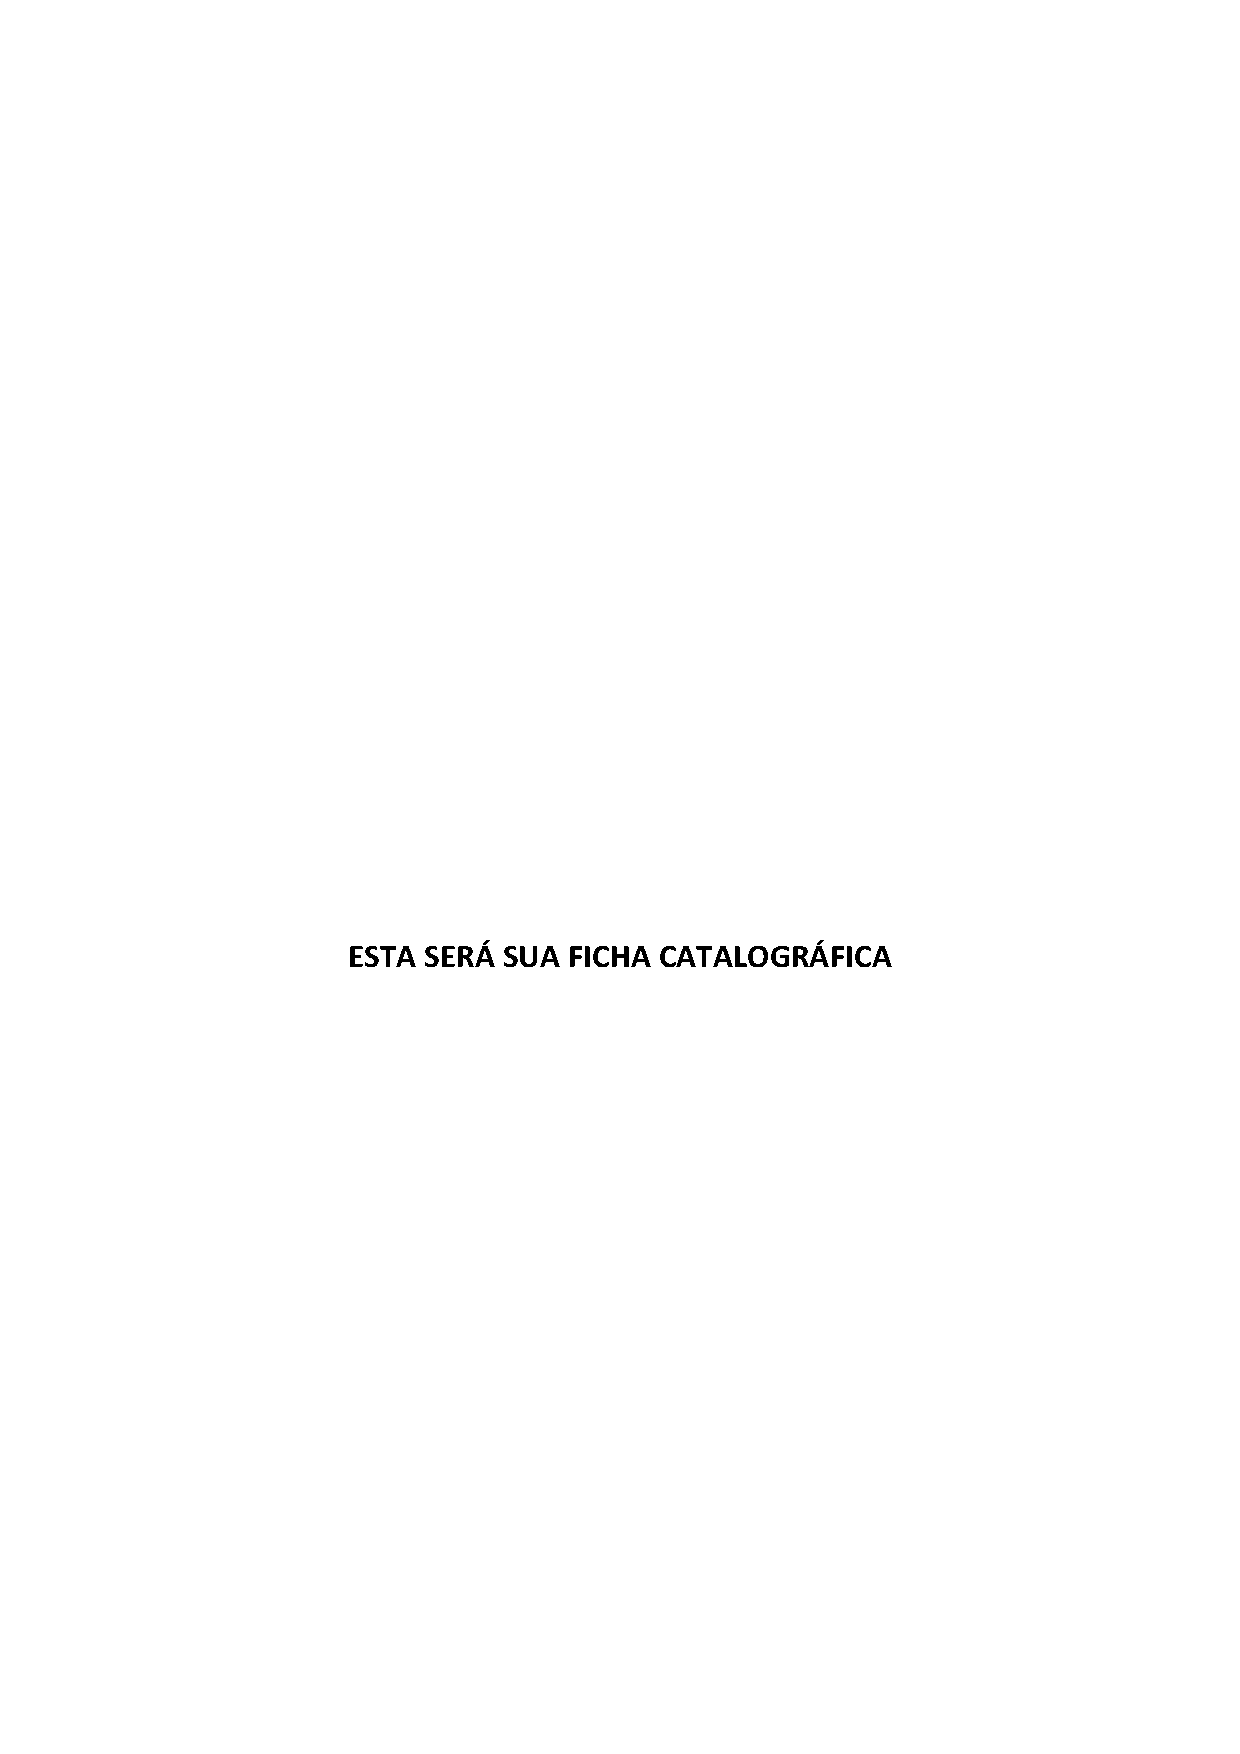
\includepdf[pages=-]{anexos/ficha.pdf}

%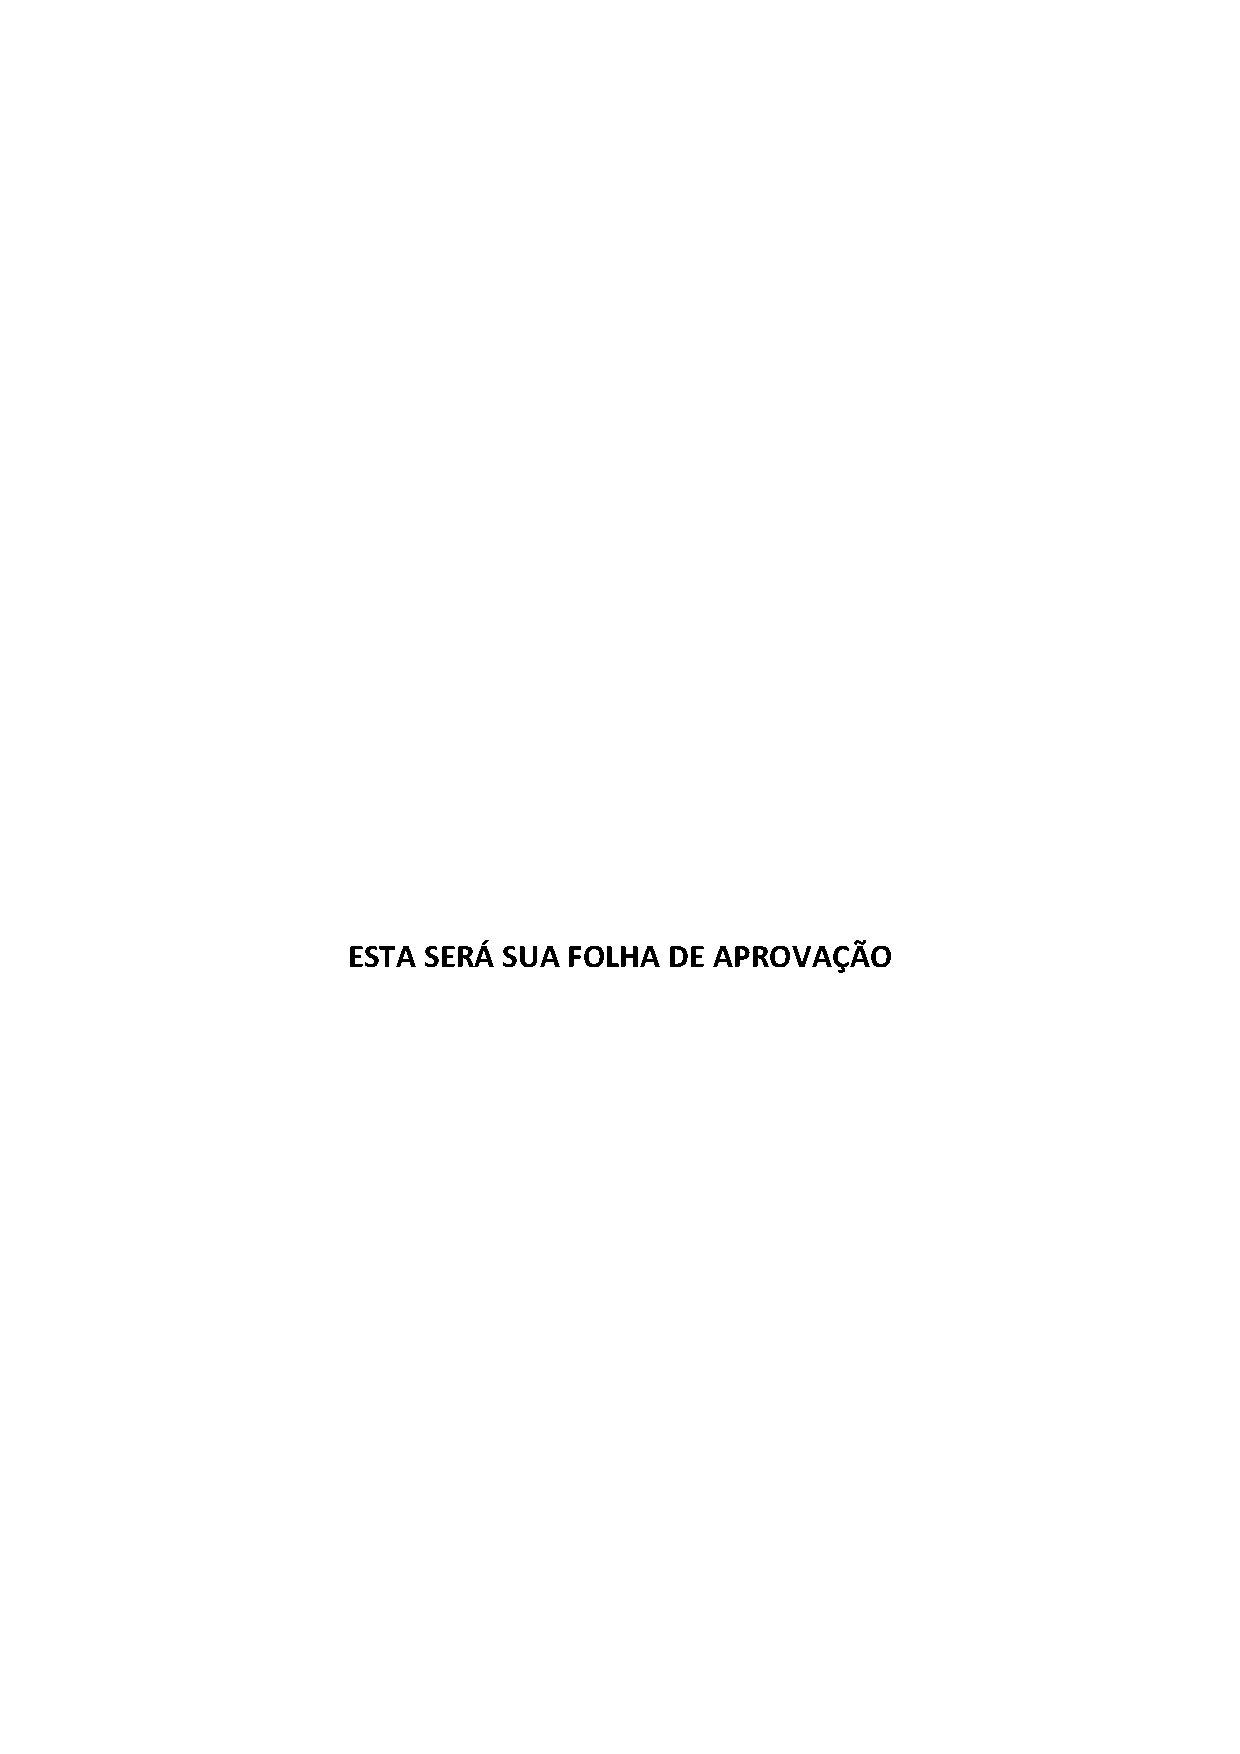
\includepdf[pages=-]{anexos/aprovacao.pdf}

\setlength{\ABNTEXsignwidth}{12cm}

%--------------------------------------------------------------------------------
% Está comentado pelo mesmo motivo da ficha catalográfica 
%--------------------------------------------------------------------------------
% \begin{folhadeaprovacao}
% 	\begin{center}
% 	    {\ABNTEXchapterfont\bfseries\large\imprimirinstituicao}
% 	    \vspace*{\fill}

% 	    {\ABNTEXchapterfont\bfseries\large FOLHA DE APROVAÇÃO}
% 	    \vspace*{\fill}

% 	    {\ABNTEXchapterfont\bfseries\large\imprimirautor}

% 	    \vspace*{\fill}\vspace*{\fill}
% 	    {\ABNTEXchapterfont\bfseries\large\imprimirtitulo}
% 	    \vspace*{\fill}

% 	    {\hspace{.45\textwidth}
% 		\begin{minipage}{.5\textwidth}
% 			\SingleSpacing
% 			\ABNTEXchapterfont\imprimirpreambulo \\ \\

% 			{\ABNTEXchapterfont\imprimirorientadorRotulo~\imprimirorientador\par}
% 			{\ABNTEXchapterfont\imprimircoorientadorRotulo~\imprimircoorientador\par}

% 		\end{minipage}%
% 	    \vspace*{\fill}}
% 	\end{center}

% 	\vspace*{\fill}

% 	\begin{center}
% 			 \ABNTEXchapterfont\large Aprovado em: \_\_\_\_ de \_\_\_\_ de 2019
% 	\end{center}

% 	\vspace*{\fill}

% 	\begin{center}
% 			 \ABNTEXchapterfont\bfseries\large Banca Examinadora
% 	\end{center}

%   \ABNTEXchapterfont\assinatura{Rosalvo Ferreira de Oliveira, Doutor, Universidade Federal do Vale do São Francisco}
% 	\ABNTEXchapterfont\assinatura{Jorge Luis Cavalcanti Ramos, Doutor, Universidade Federal do vale do São Francisco}
%  \ABNTEXchapterfont\assinatura{Ricardo Argenton Ramos, Doutor, Universidade Federal do Vale do São Francisco}
% 	 \vspace*{\fill}


% \end{folhadeaprovacao}

%--------------------------------------------------------------------------------
% Insere a epígrafe
%--------------------------------------------------------------------------------
\newpage
\begin{epigrafe}
\vspace*{\fill}
\begin{flushright}
		\textit{Planet Earth is blue and there's nothing I can do}\\
		\textbf{David Bowie}\\
		\textbf{Space Oddity}
\end{flushright}
\end{epigrafe}
%--------------------------------------------------------------------------------
% Seção de agradecimentos
%--------------------------------------------------------------------------------
\begin{agradecimentos}
	
Agradeço primeiramente a Deus e a minha família, principalmente meus pais, João
Alves e Regina Coeli, e a meus irmãos, Maria Alice e Luciano, pelo apoio e carinho
durante todo o caminho da graduação.

À minha noiva, Nathanaele, por mesmo longe se fazer presente e me incentivar a
continuar em frente sempre.

Agradeço ao ``Clubinho Guaraná'' composto por Ellen, Daniel, Talita, Carolina,
Isaac, Esron e Mauricio, pelos momentos compartilhados de alegria, estresse e,
as vezes, tristeza. Um grupo não só de leitura, mas de colaboração mútua e
respeito. Um agradecimento especial a Ellen por estar comigo desde o começo da
jornada.

Agradeço a meu orientador, Rosalvo, por me apresentar a oportunidade de dar
inicio oa projeto FutVasf2D e trabalhando comigo por 2 anos seguidos até
finalmente a conclusão.

Obrigado aos professores Ricardo Ramos e Jorge Cavalcanti que contribuíram com a
melhoria deste trabalho.

Obrigado ainda a Brauliro e Ricardo, novamente, com conselhos profissionais e
acadêmicos que contribuíram para formação e ofereceram momentos de lazer que se mostraram
um óasis em meio a todo o estresse do curso, se tornando amigos, ouso dizer.

Obrigado à Deise por sempre ajudar com toda a burocracia da UNIVASF, até quando
parecia que não tinha jeito.

Por fim agradeço a todos que estiveram comigo neste caminho, professores,
colegas e amigos. Obrigado por me ajudar a me tornar quem eu sou hoje.

\end{agradecimentos}

%--------------------------------------------------------------------------------
% Insere a segunda epígrafe
%--------------------------------------------------------------------------------
% \begin{epigrafe}
%     \vspace*{\fill}
% 	\begin{flushright}
% 		Se pude enxergar a tão grande distância, foi subindo nos ombros de gigantes.\\
% 		 \vspace{\baselineskip}
% 		\textbf{Isaac Newton}\\
% 		\textbf{Carta à Robert Hooke, 1676}
% 	\end{flushright}
% \end{epigrafe}



%--------------------------------------------------------------------------------
% Seção de resumos
%--------------------------------------------------------------------------------
% resumo em português
\setlength{\absparsep}{18pt} % ajusta o espaçamento dos parágrafos do resumo
\begin{resumo}

% Em geral o resumo precisa das seguintes partes [contexto], [problema],
% [solução/objetivo], [metodologia], [validação/experimento] e [resultados].

Este trabalho se debruça sobre a copa do mundo de futebol de robôs
(\textit{RoboCup Soccer}), que incentiva a produção de pesquisas na área de
inteligência artificial e robótica, enquanto parte do projeto FutVasf2D que
busca o desenvolvimento de um time oficial de futebol de robôs na liga de
simulação 2D para UNIVASF, investigando o efeito de diferentes modelos
de mundo aplicados à técnica de aprendizado por reforço \textit{Q-Learning}
sobre a performance do time na posição de defesa. Este trabalho busca encontrar
modelos que facilitem o aprendizado dos agentes na tentativa de interceptar
bolas lançadas pelo adversário e de capturar a bola em posse do adversário. Para
alcançar o objetivo foram desenvolvidos modelos através de diferentes
combinações de estados, ações, recompensas e métodos de implementação. Os
modelos foram treinados e avaliados através da ferramenta HFO que cria situações
de defesas aleatoriamente agilizando o processo de treinamento. Os resultados
encontrados foram comparados entre si e entre o time base original
(\textit{WrightEagleBASE}), mas apresentaram desempenho abaixo do esperado,
levando discussões de possíveis falhas no processo.


 \textbf{Palavras-chave}: Futebol de Robôs, Aprendizado por reforço, \textit{Q-Learning}, \textit{RoboCup Simulation 2D}, Defesa.

\end{resumo}

%---------------------------------------------------------------------------------
% resumo em inglês
\begin{resumo}[Abstract]
\begin{otherlanguage*}{english}

	This work dwell on the soccer world cup (RoboCup Soccer), which encourages
	researchers in the artificial intelligence and robotics fields, being part
	of the FutVasf2D project that looks for the development of an official robot
	soccer team in the 2d simulation league to the UNIVASF, investigating the
	effects of different world designs applied to the reinforcement technique
	Q-Learning about the performance of the team in defense position. This work
	tries to find designs that improve the learning of the agents into trying to
	intercept balls launched by the adversaries and capture the ball in the
	opponent possession. To reach this objective designs with differents
	combination of states, actions, rewards and implementation methods were
	developed. The designs were trained e evaluated through the HFO tools, which
	creates situations of defense randomly making the learning process faster.
	The found results were compared between themselves and the original base
	team (WrightEagleBASE), but showed performance below the expected, leading
	to discussions about the possible faults in the process.
	
	\vspace{\onelineskip}

	\noindent
	\textbf{Key-words}: \textit{Robot Soccer, Reinforcement Learning, Q-Learning, RoboCup Simulation 2D, Defense}.

\end{otherlanguage*}
\end{resumo}


%---------------------------------------------------------------------------------
% Insere lista de ilustrações
%---------------------------------------------------------------------------------
\begin{KeepFromToc} % Este comando evita que todas as seções dentro dele de apareçam no sumário
\pdfbookmark[0]{\listfigurename}{lof}
\listoffigures
%\addcontentsline{toc}{chapter}{Lista de Figuras}
\cleardoublepage


%---------------------------------------------------------------------------------
% Insere lista de tabelas
%---------------------------------------------------------------------------------
\pdfbookmark[0]{\listtablename}{lot}
\listoftables
\cleardoublepage

%---------------------------------------------------------------------------------
% Ajusta lista de código - alterar de figures para códigos - by @Gabrielr2508
%---------------------------------------------------------------------------------
\makeatletter
\let\l@listing\l@figure
\def\newfloat@listoflisting@hook{\let\figurename\listingname}
\makeatother

%---------------------------------------------------------------------------------
% Insere lista de códigos - by @leolleocomp
%---------------------------------------------------------------------------------
\listoflistings

\end{KeepFromToc}

%---------------------------------------------------------------------------------
% Insere lista de abreviaturas e siglas
%---------------------------------------------------------------------------------
\begin{siglas}
	\item[CBR] Competição Brasileira de Robótica
    \item[CMAC] Computador Aritmético de Modelo Cerebelar
    \item[DCBD] Descoberta de Conhecimento em Base de Dados 
    \item[HAQL] \textit{Q-Learning} Acelerado Heuristicamente
    \item[HFO] Ofensa de Meio Campo
    \item[KDD] Descoberta de Conhecimento em Base de Dados, do inglês \textit{Knowledge Discovery in Databases}
    \item[MDP] Processo de Decisão Markoviano
    \item[PIBIC] Programa Institucional de Bolsas de Iniciação Científica 
    \item[QRL] Aprendizado por Reforço Qualitativo
    \item[QSR] Raciocínio Espacial Qualitativo
    \item[RPROP] \textit{Backpropagation} Resiliente
    \item[SARSA] Estado-Ação-Recompensa-Estado-Ação
    \item[UNIVASF] Universidade Federal do Vale do São Francisco
	    
\end{siglas}

%---------------------------------------------------------------------------------
% Insere o sumario
%---------------------------------------------------------------------------------
\pdfbookmark[0]{\contentsname}{toc} 
\tableofcontents*
\cleardoublepage


	\textual
		\pagestyle{simple}
		%--------------------------------------------------------------------------------------
% Este arquivo contém a sua introdução, objetivos e organização do trabalho
%--------------------------------------------------------------------------------------
\chapter{Introdução}

Como descrito por \citeonline{kitano1997robocup}, a \textit{RoboCup}, a copa do mundo de futebol de
robôs, procura fomentar as pesquisas acerca de robótica e inteligência artificial fornecendo um
problema padrão capaz de avaliar teorias, algoritmos e arquiteturas de agentes. O projeto da
\textit{RoboCup} é dividido em várias ligas, desde robôs humanoides até a liga de simulação 2D.
Proporcionando assim, um ambiente criativo e desafiador para que novas tecnologias sejam criadas e
aplicadas por alunos de graduação.

Segundo \citeonline{henn2017optimizing}, a liga de simulação 2D representa um jogo de futebol, em um
\textit{framework} multiagente, no qual o ambiente é um campo de futebol em duas dimensões e os
agentes são os jogadores, criando a vantagem de livrar os pesquisadores de toda a parte mecânica e
eletrônica para que o foco se volte à análise de dados e construção da estratégia.
\citeonline{henn2017optimizing} ainda afirmam que a principal parte da liga é a modelagem de uma
estratégia ou método efetivo o suficiente para obter performance superior aos adversários. Por fim,
os autores relatam que uma das estratégias com melhores resultados é a utilização de agentes
inteligêntes.

De acordo com \citeonline{russell2016artificial}, um agente inteligente é tudo o que pode ser
considerado capaz de perceber seu ambiente por meio de sensores e de agir sobre seu ambiente por
intermédio de atuadores. A Figura \ref{img:agent} ilustra a arquitetura clássica de um agente, onde
é possível perceber que o agente interage com o ambiente por meio de sensores e atuadores.

\imagem{0.5}{agent}{Arquitetura geral de um agente.}{\cite{russell2016artificial}}

No domínio da liga de simulação 2D da \textit{RoboCup}, o ambiente é composto pela representação 2D
do campo, as traves, a bola e os jogadores. Esse ambiente é captado pelos agentes através dos seus
sensores classificados como físicos, visuais ou acústicos, que, respectivamente, servem para
perceber o estado do agente, referente ao vigor, velocidade e posição; as posições e velocidades dos
demais objetos no ambiente, incluindo jogadores e mensagens oriundas dos aliados. Os atuadores dos
agentes correspondem aos mecanismos de movimento, rotação e chute
\cite{robocupfederationofficialwebsite}. Um dos aspectos que torna o desenvolvimento de agentes
inteligentes para jogos de futebol de robôs desafiador é a  característica de seu ambiente:

\begin{itemize}
    \item \textbf{Parcialmente observável}: O ambiente para um agente jogador de futebol de robôs é
    parcialmente observável, pois os seus sensores são imprecisos e também porque partes do estado
    estão simplesmente ausentes nos dados do sensor \cite{schmill2000learning};
    
    \item \textbf{Estocástico}: De acordo com \citeonline{hayes1995architecture}, se o próximo
    estado do ambiente é completamente determinado pelo estado atual e pela ação executada pelo
    agente, dizemos que o ambiente é determinístico; caso contrário, ele é estocástico. Desta forma,
    o ambiente para um agente jogador de futebol de robôs é estocástico, pois o próximo estado não
    depende apenas da sua ação;
    
    \item \textbf{Episódico}: Em um ambiente de tarefa episódico, a experiência do agente é dividida
    em episódios atômicos \cite{wooldridge2001intelligent}. Cada episódio consiste na percepção do
    agente, e depois na execução de uma única ação. É crucial que o episódio seguinte não dependa
    das ações executadas em episódios anteriores. Desta forma, o ambiente de tarefa para o agente
    jogador de futebol de robôs é episódico;
    
    \item \textbf{Dinâmico}: Ambientes estáticos são fáceis de manipular, porque o agente não
    precisa continuar a observar o mundo enquanto está decidindo sobre a realização de uma ação, nem
    precisa se preocupar com a passagem do tempo. No entanto, o ambiente de tarefa para o agente
    jogador de futebol de robôs é dinâmico, pois o ambiente pode ser alterado enquanto o agente está
    deliberando \cite{franklin1996agent};
    
    \item \textbf{Multiagente}: Um ambiente ainda pode ser classificado como agente único e
    multiagente. Agente único não existem outros agentes que utilizam a mesma medida de performance,
    como exemplo podemos citar: um agente que resolve um jogo de palavras cruzadas sozinho está
    claramente em um ambiente de agente único, enquanto que um agente jogador de futebol de robôs
    está em ambiente multiagente, tanto cooperativo (agentes do mesmo time) como também competitivos
    (agentes do time adversário) \cite{poggi1996multi}. 

\end{itemize}

\section{Motivação}

FutVasf2D é um projeto que nasceu em 2017 com auxílio do Programa Institucional de Bolsas de
Iniciação Científica (PIBIC) para o desenvolvimento de um time oficial de futebol robôs para
Universidade Federal do Vale do São Francisco (UNIVASF) na categoria de simulação 2D. O primeiro
trabalho do projeto teve como objetivo o desenvolvimento de um módulo de decisão para o momento do
chute a gol. O projeto está tendo continuidade com, além do presente trabalho, outro PIBIC que visa
o desenvolvimento de um módulo de passes.

Durante o processo de desenvolvimento deste trabalho almeja-se por em prática conhecimentos tratados
 forma téorica na área de aprendizado de máquinas enfrentando o desafio da aplicação das técnicas
 tratadas em um ambiente complexo e prático. A técnica de aprendizado por reforço aplicada neste
 trabalho é a \textit{Q-Learning} devido ao fato desta ser uma técnica comum e já utilizada por
 diversos trabalhos na área.

Com o término deste trabalho espera-se a participação do time desenvolvido na Competição
Brasileira de Robótica (CBR) como meio de divulgar o projeto e angariar interessados no
desenvolvimento de novas estratégias e melhoramento das já desenvolvidas no meio acadêmico da
UNIVASF.

\section{Definição do Problema}

De acordo com \citeonline{oliveira2009data}, uma partida de futebol apresenta situações que exigem
dos jogadores a tomada de decisão acerca da ação a ser tomada. Quando um jogador está com a bola,
por exemplo, ele deve decidir se deve passar a bola para um aliado, driblar um adversário ou chutar
a bola para o gol. Todas essas ações são decididas através de avaliações do conhecimento acerca da
situação atual do jogo. O mesmo pode ser afirmado para situações onde o time adversário está com
posse de bola, neste caso, os jogadores devem sempre tomar a melhor decisão com base no estado atual
para evitar sofrer gol e recuperar a posse de bola do adversário.

Alguns times que competem ou competiram em campeonatos da liga fornecem código-fonte de times,
chamados de times bases, a fim de facilitar o desenvolvimento de novos times para novos competidores. É
o caso dos times HELIOS, do Japão, que fornece o time base Agent2D\footnote{http://rctools.osdn.jp/pukiwiki/} ou o WrightEagle, da China,
que fornece o WrightEagleBASE\footnote{https://wrighteagle2d.github.io/}, utilizado neste projeto. Tais times são desenvolvidos com estratégias
simples para que possam ser melhoradas pelas novas equipes.

\citeonline{gabel2008case} afirmam que o uso de técnicas de aprendizagem para o desenvolvimento da
capacidade defensiva de um time vêm sendo quase negligenciadas, de forma que as pesquisas focam, em
sua maioria, em tarefas como a de passe, chute a gol ou posicionamento do jogador com posse de bola.

Ainda segundo \citeonline{gabel2008case}, estratégias de defesa são divididas em 2 partes, o
posicionamento dos jogadores de forma a melhor interceptar passes ou tentativas de chute ou marcar
oponentes, e o de atacar o jogador com posse de bola a fim de obtê-la.

Neste trabalho, serão levadas em conta ambas as facetas das estratégias de defesa, de forma que o
problema proposto pode ser definido como a identificação de melhor ação a ser tomada, utilizando
dados obtidos do ambiente através de seus sensores, entre:

\begin{itemize}
    \item Mover-se para uma melhor posição;
    \item Marcar um jogador adversário; 
    \item Interceptar a bola e
    \item Bloquear avanço do jogador com posse de bola.
\end{itemize}

\section{Objetivos}

\subsection{Objetivo Geral}

Investigar performance de modelos no desenvolvimento de módulo responsável por tomar decisões
voltadas para defesa para o time de futebol de robôs da liga de simulação 2D FutVasf2D utilizando a
técnica de aprendizado por reforço \textit{Q-Learning}.

\subsection{Objetivos Específicos}

\begin{enumerate}
    \item Desenvolver modelos aptos a representar o ambiente do futebol de robôs da liga de
    simulação 2D em algoritmos de aprendizado por reforço aplicados na solução do problema proposto;
    
    \item Implementar os modelos propostos no algoritmo \textit{Q-Learning} no time
    \textit{WrightEagleBASE}, usado como base para o FutVasf2D;
    
    \item Treinar os times implementados através da execução de partidas com situações controladas;
    
    \item Comparar resultados e identificar e falhas e melhorias.
\end{enumerate}

\section{Organização do Trabalho}

Além do presente capítulo, Introdução, estão presentes neste trabalho 3 capítulos, Fundamentação
Teórica (\ref{sec:fundamentation}), Materiais e Métodos (\ref{sec:newModule}), Resultados
(\ref{sec:results}), Conclusão (\ref{sec:conclusion}) e Trabalhos Futuros (\ref{sec:future}).

O Capítulo \ref{sec:fundamentation} fundamenta teoricamente o trabalho apresentando na Seção
\ref{trabalhosRelacionados} trabalhos relacionados que reforçam a metodologia por trás da execução
deste, a Seção \ref{aprendizado} explana o conceito e funcionamento do aprendizado por reforço e, na
Subseção \ref{qlearning}, faz o mesmo com o algoritmo \textit{Q-Learning}, ponto fundamental para o
desenvolvimento deste trabalho.

O Capítulo \ref{sec:newModule} explica o processo proposto para o desenvolvimento dos modelos e
coleta de resultados. Na Seção \ref{modelagem} é exposto o conceito de modelagem do ambiente e seus
desafios. A Seção \ref{implementacao} explica o processo de implementação e as
variações aplicadas, enquanto a Seção \ref{meotodologia}, é acerca da metodologia
experimental, como o treinamento e a forma de avaliação.

O Capítulo \ref{sec:results} apresenta a descrição dos modelos desenvolvidos, a fundamentação de
cada um e os resultados obtidos em seus respectivos treinamentos.

No Capítulo final \ref{sec:conclusion} constam as devidas conclusões tomadas a partir do processo de
desenvolvimento deste trabalho e dos resultados obtidos pelos experimentos, procurando responder
indagações oriundas da análise dos dados do capítulo anterior. Também é
trabalhado na Seção \ref{sec:future}, o traçado de uma continuidade
para o projeto iniciado apresentando propostas de novas investigações e o caminho a ser tomado.
		%--------------------------------------------------------------------------------------
% Este arquivo contém a sua funtamentação teórica
%--------------------------------------------------------------------------------------
\chapter{Fundamentação Teórica}\label{sec:fundamentation}

\section{Trabalhos Relacionados}\label{trabalhosRelacionados}

Diversos trabalhos foram redigidos utilizando aprendizado por reforço no domínio da \textit{RoboCup
Soccer Simulation 2D}, cada um desses trabalhos apresentam modelagens diferentes para o mundo.

A modelagem de mundo é a forma como o ambiente é representado, ou simulado. Um agente inteligente
precisa constantemente entender como está o ambiente no qual ele está inserido, por isso é
importante a definição da representação do mundo de forma que melhor se adéque ao processo de
aprendizado do agente.

Um agente empregado no aprendizado do jogo-da-velha, pode ser utilizado com exemplo. O agente
precisa entender como o jogo está sendo encaminhado para que o mesmo possa decidir em que posição
jogar, porém, o agente isolado não tem acesso ao estado do jogo e precisa de uma representação do
mesmo para que possa entende-lo. Uma abordagem válida é numerar o tabuleiro conforme a Figura
\ref{img:ticTacToeNumbers} e atrelar a cada célula um valor que varia de acordo com o que é marcado
na mesma, uma escolha razoável é atribuir o valor ``$-1$'' à células preenchidas pelo jogador
adversário, ``$0$'' à células não preenchidas e ``$1$'' às preenchidas pelo próprio agente. Nota-se que com
essa representação o agente consegue perceber em que situação se encontra e assim escolher uma ação.
Podemos chamar cada uma das células de variável, já que nelas se encontram os valores que determinam
qual o estado atual do ambiente.

\imagem{0.6}{ticTacToeNumbers}{Representação do tabuleiro de jogo-da-velha.}{O Autor}

É fácil encontrar exemplos de problemas inseridos em ambientes que são mais complexos que o citado.
Para esses problemas é comum encontrar variáveis de valores contínuos, nesses casos é necessário
pensar em como representar as variáveis de forma discreta para que seja possível se obter um número
finito de estados. Alguns dos trabalhos citados adiante demonstram maneiras de interpretar os dados
do ambiente para que possa ser aplicada técnica de aprendizado. 

\citeonline{gabel2008case} desenvolveram jogadores de defesa com comportamento agressivo, ou seja,
jogadores que interferem e tentam tomar a bola do jogador adversário, utilizando aprendizado por
reforço. O algoritmo desenvolvido foi chamado de NeuroHassle e utiliza redes neurais e uma abstração
do mundo em 9 dimensões, distância entre o jogador e oponente com posse de bola; vetor de velocidade
do jogador; velocidade absoluta do oponente com posse de bola; vetor de posicionamento da bola;
ângulo do corpo do jogador em relação ao oponente com posse de bola; ângulo do corpo do adversário
em relação ao gol aliado; ângulo definido pela posição do gol aliado, a posição do oponente com
posse de bola e a posição do jogador. O treinamento foi feito de forma episódica em partidas de
competições anteriores. O time gerado obteve uma taxa de falha menor que 20\% e, em competição,
cerca de 30 tomadas de bola por partida.

Uma variação de redes neurais com a utilização de \textit{backpropagation}, chamada de
\textit{Backpropagation} Resiliente (RPROP, do inglês \textit{Resilient Backpropagation}), foi
utilizada por \citeonline{Riedmiller2005Brainstormers2D} no treinamento de jogadores sem posse de
bola ao mesmo tempo que a escolha de ações do jogador com posse de bola. Para isto foi feita uma
discretização do domínio em um Processo de Decisão Markoviano (MDP, do inglês \textit{Markovian
Decision Process}) que destacou as variáveis posição e velocidade da bola e a posição de todos os
atacantes aliados e defensores adversários, além das possíveis ações, que para os jogadores com
posse de bola consistem em passar a bola diretamente para um aliado, lançar a bola de forma que um
aliado possa interceptar a bola antes de um adversário e driblar, já para os jogadores sem posse de
bola, é possível se mover em 8 direções a partir do local atual ou a partir do local inicial ou
mover-se para o local inicial. Este trabalho resultou no time vencedor do ano de 2007 da liga de
simulação 2D da \textit{RoboCup Soccer}.

A técnica \textit{Q-Learning} é aplicada em alguns trabalhos, como o de
\citeonline{neri2012proposal}, que utiliza desta técnica a fim de obter um sistema de tomada de
decisões focado no ataque. Nesse trabalho, os estados foram discretizados em 7 estados,
caracterizados como quando é possível lançar a bola para um aliado melhor posicionado; um adversário
mais próximo está atrás do jogador com posse de bola; o adversário mais próximo está a mais de 7
metros; o adversário mais próximo está a uma distância entre 7 e 6 metros; o adversário mais próximo
está a uma distância entre 6 e 5 metros; o adversário mais próximo está a uma distância menor de 4
metros e há uma linha direta entre o jogador com posse de bola e o gol adversário. Além disso, 7
ações podem ser tomadas, são elas, passar a bola para um jogador mais próximo do gol adversário,
avançar devagar, avançar rapidamente, passar a bola para um jogador próximo, driblar, segurar a bola
ou chutar ao gol.

O modelo foi treinado e testado através da execução de conjuntos de 10 partidas. O conjunto de
treinamento se  deu contra o time base do Helios apenas na situação de posse de bola. Após o
treinamento, o time foi tuilizado no primeiro conjunto de testes contra o time base do Helios, além
disso, outro foiexecutado entre Helios e o PetSoccer, além de um entre o time treinado e o PetSoccer
para comparação, e por fim outro contra o time chinês WrightEagles. No primeiro conjunto foram
realizados 6 gols contra o Helios, o Helios executou 47 gols contra o PetSoccer, o time treinado
conseguiu 61  gols contra o PetSoccer e 6 contra o WrightEagles. Mostrando que a utilização do
\textit{Q-Learning} resultou numa melhoria, ganhando a maioria dos jogos. A mesma técnica foi
utilizada no time brasileiro GPR-2D de 2012, descrito em \citeonline{neriteam}, com o objetivo de
treinar a tomada de decisão para quando o jogador estiver com posse de bola. O time foi classificado
e chegou a segunda fase do campeonato mundial da \textit{RoboCup Soccer Simulation 2D}.

\citeauthoronline{liu2008regional} (\citeyear{liu2008regional} e \citeyear{liu2009sparse}), utilizam
\textit{Q-Learning} com uma abstração do conjunto de agentes como um grande agente e o conjunto de
suas ações como uma ação deste grande agente chamando os dois algoritmos criados de \textit{Regional
Cooperative Q-Learning} e \textit{Sparse Cooperative Q-Learning} (\textit{Q-Learning} Cooperativo
Regional e \textit{Q-Learning} Cooperativo Esparso). Nesses trabalhos foram identificados estados
onde não é necessário que as ações sejam decididas em conjunto (não coordenados) e onde é
(coordenados), utilizando uma abordagem baseado em campos potenciais. Na abordagem regional foram
encontrados 5012 estados coordenados e 34390 não coordenados, já na abordagem esparsa, foram 4720
coordenados e 34682 não coordenados. O modelo foi treinado  com uma simplificação de partidas com
dois agentes defendendo e um adversário atacando e a região (reduzida para 40 x 20) dividida em 200
células. Foram rodados experimentos com 200000 e 500000 episódios comparando a técnica aplicada com
a técnica MDP e a linear independente. Para 200000 episódios foi obtida uma média de tempo de
captura de 6,57 segundos para a abordagem regional e 6,49 para a esparsa, mostrando-se o melhor
dentre 3 métodos enquanto com 500000 episódios apresenta uma média de 6,49 segundos na abordagem
regional e 6,40 na abordagem esparsa, maior apenas que o do método MDP que apresentou 6,23 segundos.

Alguns trabalhos utilizam variações do \textit{Q-Learning}, como
\citeonline{carvalho2011reinforcement}, que desenvolveu um módulo de drible unindo Computador
Aritmético de Modelo Cerebelar (CMAC, do inglês \textit{Cerebellar Model Arithmetic Computer}) e
Estado-Ação-Recompensa-Estado-Ação (SARSA, do inglês \textit{State-Action-Reward-State-Action}),
este último algoritmo foi concebido como \textit{Q-Learning} conexionista modificado. Neste trabalho
a tarefa de drible foi mapeada como um problema episódico adequado para o trabalho com aprendizado
por reforço onde foram destacadas duas ações primitivas, segurar a bola e driblar (que consiste em
girar o corpo a uma determinada angulação, chutar a bola a uma distância determinada e correr para
interceptá-la) e as seguintes variáveis para compor um estado para o jogador que deverá driblar, o
ângulo global de um objeto, o ângulo relativo entre dois objetos, a distância entre dois objetos, a
altura e largura do campo e se o jogador está perto do topo ou da parte mais baixa do campo. O
treinamento do modelo criado foi feito em 5 experimentos de 50000 episódios nos quais o jogadores
não podiam recuperar a \textit{stamina} por si só utilizando o ambiente padrão e um ambiente de
treino de 20 x 20. Para testar foram executados 10000 cenários com configurações aleatórias. No fim
do treinamento foi obtido um número de vitórias de cerca de 53\% e 58\% dos testes pós-treino.

O SARSA também foi empregado em \citeonline{homem2017improving} em conjunto com o Raciocínio
Espacial Qualitativo (QSR, do inglês \textit{Qualitative Spatial Reasoning}), chamando o resultado
de Aprendizado por Reforço Qualitativo (QRL, do inglês \textit{Qualitative Reinforcement Learning})
e aplicou no desenvolvimento de um mecanismo de ataque para um time de simulação 2D. Para alcançar o
objetivo foi utilizado o formalismo eOPRAm para discretizar o mundo em regiões qualitativas pelo
qual foram identificadas um total de 14 variáveis, são elas a posição e orientação do jogador, a
distância e ângulo do jogador em relação à bola, se o jogador pode ou não chutar, distância e ângulo
do jogador em relação ao gol adversário, maior ângulo aberto para o gol, distância entre os aliados
e o adversário mais próximo, maior ângulo aberto para passe para cada aliado, numeração de cada
aliado e de cada adversário.

As possíveis ações foram definidas como driblar, chutar e passar a bola para um aliado especifico. O
treinamento foi realizado utilizando a ferramenta Ofensa de Meio Campo (HFO, do inglês
\textit{Half-Field Offense}) 30 vezes de forma independente com 1000 episódios em 3 situações
diferentes, a primeira com apenas um jogador atacando sem nenhuma defesa, a segunda com apenas o
atacante e o goleiro e a terceira com o atacante, o goleiro e um zagueiro. Foi realizada uma
comparação da técnica utilizada com a abordagem quantitativa utilizando análise de variância. Na
primeira situação o resultado foi de uma média de 99,3\% de gols se mostrando melhor que a
quantitativa com certeza de 95\%, enquanto a segunda e terceira situação se mostraram melhor com
margem de 1\% com 81,2\% e 47,6\% contra 78,3\% e 40,6\% respectivamente.

Além dessas variações, algumas foram empregadas com o intuito de acelerar o aprendizado, este foi o
caso de \citeonline{celiberto2007heuristic} e \citeonline{bianchi2010case}. O primeiro, utilizou a chamada \textit{Q-Learning} Acelerado Heuristicamente (HAQL, do inglês
\textit{Heuristically Accelerated Q-Learning}) para treinar um goleiro e jogador de defesa. Para
tanto, foi identificada uma heurística aplicável ao domínio e implementada no algoritmo
\textit{Q-Learning} ao mesmo tempo que é feita a discretização do mundo. As variáveis de estado para
o algoritmo foram a posição dos agentes e da bola numa grade e a direção para a qual o agente está
virado definida por norte, sul, leste ou oeste. As ações que podem ser tomadas são mudar a direção
para a qual o agente está virado para um objeto especifico, mover em direção a bola, mover-se com a
bola, passar a bola para o goleiro, chutar a bola para longe do gol mover-se para perto de um
oponente. Foram executadas 10 sessões de treinamento para o algoritmo criado, \textit{Q-Learning}
puro e a função heurística pura com 100 episódios cada, onde cada episódio consiste de uma partida
de 3000 ciclos. Foi analisada a curva de aprendizado e o número de gols sofridos para cada
algoritmo. E utilizado o teste \textit{t-student} que validou a hipótese de que a aplicação de
heurística no \textit{Q-Learning} acelera o aprendizado com nível de confiança de 95\% e uma taxa de
gols sofridos menor que as demais opções testadas.

Já \citeonline{bianchi2010case}, utilizam heurística baseada em casos para acelerar o
\textit{Minmax-Q}, que também é uma variação do \textit{Q-Learning}, para melhorar a tomada de
decisões. Os casos destacado para utilização no algoritmo foram o de que caso o jogador esteja com a
bola e não exista adversário no caminho, avança para o gol; se houver um adversário bloqueando, mova
para cima ou para baixo; se houver um aliado mais próximo do gol, passa a bola e se o adversário
estiver com a bola e o jogador estiver próximo, fica na frente do adversário. O treinamento foi
feito com 20000 jogos de 10 tentativas em um domínio chamado ``futebol expandido de Littman''.
Chegou-se ao resultado de que a solução encontrada não é ótima, mas a hipótese de que o aprendizado
é acelerado foi comprovado, através do teste de \textit{t-student} e uma comparação dos resultados
das partidas e das curvas de aprendizado.

Diante dos exemplos apresentados e considerando a natureza do problema, fica decidido utilizar uma
técnica de aprendizado por reforço, mais especificamente \textit{Q-Learning}, para o treinamento de
um modelo de tomada de decisões de defesa do time em desenvolvimento, \textit{FutVasf2D}.

\section{Aprendizado por Reforço}\label{aprendizado}

Segundo \citeonline{shalev2014understanding}, aprendizado por reforço é uma técnica de aprendizado
intermediária, entre supervisionado e não supervisionado, onde o agente precisa realizar mais
previsões durante os ``testes''.

\citeonline{russell2016artificial} afirmam que aprendizado por reforço é necessário quando não há um
bom ''professor`` para a tarefa a ser executada. Apontam ainda que, através de ações aleatórias, o
modelo é capaz de ``aprender'' a realizar predições sobre o ambiente. Logo, o papel do aprendizado
por reforço é, utilizando-se de recompensas, encontrar uma função eficaz para o agente.

Uma analogia apontada por \citeonline{russell2016artificial} é a que compara o aprendizado por
reforço com a forma que seres vivos aprendem. Animais são capazes de perceber quando especificas
sensações são recompensas positivas ou negativas e essa é uma característica que facilita o
adestramento de cães, por exemplo, no qual o cão consegue entender que fez algo positivo através de
recompensas como petiscos ou carinho ou negativo como a repreensão em determinado tom de voz.

\begin{citacao}
    Aprendizado por reforço é aprender o que fazer - como mapear situações em ações - de forma a
    maximizar uma recompensa numérica. Aquele que aprende não é informado quais ações tomar, no
    entanto, deve descobrir quais ações resultam em uma maior recompensa tentando executá-las.
    \cite{sutton2018reinforcement}
\end{citacao}

Segundo \citeonline{sutton2018reinforcement}, existem alguns elementos que devem ser conceituados em
prol de melhor entender o aprendizado por reforço, são eles, política, sinal de recompensa, função
valor e modelo de ambiente.

\begin{itemize}
    \item \textbf{Política} é o que define a forma como o agente deve se comportar em determinado
    momento. É um mapeamento entre os possíveis estados do ambiente e ações.
    
    \item \textbf{Sinal de recompensa} é um valor numérico que define o quão determinada ação afeta
    de forma positiva ou negativa na tentativa de alcançar o objetivo.
    
    \item \textbf{Função de valor} se refere ao que o agente espera acumular de recompensa no
    futuro. É como a função de recompensa, porém, ao invés de um valor imediato, retorna um valor
    para um intervalo de tempo maior.
    
    \item \textbf{Modelo de ambiente} é uma simulação do ambiente que permite  que sejam feitas
    interferências em como o ambiente se comportará. Modelos são usados para prever como estará o
    ambiente sem precisar altera-lo de fato para melhor planejar as ações.
\end{itemize}

A Figura \ref{img:reinforcement} resume o funcionamento do aprendizado por reforço como o já dito.

\imagem{0.8}{reinforcement}{Aprendizado por reforço.}{O Autor}

\citeonline{russell2016artificial} descrevem como o aprendizado por reforço pode variar, tanto em
relação ao tipo de ambiente quanto ao agente:

\begin{itemize}
    \item O ambiente pode ser acessível ou inacessível. No primeiro caso o agente consegue detectar
    o estado do ambiente através de sensores, enquanto que em ambientes inacessíveis o agente
    precisa manter e atualizar um estado interno.
    
    \item O agente pode saber \textit{a priori} sobre os estados do ambiente e como suas ações podem
    interferir no mesmo ou pode ter que aprender essas informações durante o treinamento.
    
    \item Recompensas podem ser recebidas em qualquer estado ou apenas em estados terminais.
    
    \item Recompensas podem ser valores que o modelo tenta maximizar existentes no sistema, como
    pontuação num jogo de tênis de mesa, ou valores simbólicos que funcionam como ``dicas'' de quão
    bem o agente está indo.
    
    \item Os agentes podem ser passivos ou ativos quanto a aprendizagem. Os agentes passivos apenas
    observam o ambiente mudar e tenta entender o valor de estar em vários estados, enquanto o ativo
    age conforme aprende e pode usar o gerador do problema para explorar estados desconhecidos.
\end{itemize}

\citeonline{sutton2018reinforcement} afirmam que o aprendizado por reforço depende bastante do
conceito de estado e o conceito de estado aplicado neste domínio é o estado de um MDP. Ainda segundo
\citeonline{sutton2018reinforcement}, MDP é uma forma idealizada matematicamente de um problema de
aprendizado por reforço para o qual é possível realizar declarações teóricas precisas.

Em geral, \citeonline{chan2006optimum} definem MDP como uma quádrupla $(S, K, R, T)$, onde $S$ é o
conjunto finito de possíveis estados, $K$ é o conjunto finito de possíveis ações a se tomar, $R$ é o
conjunto de recompensas imediatas para cada relação estado-ação e $T$ é o conjunto de probabilidades
de transições para cada relação estado-ação. 

Existem diversos \textit{designs} básicos para os agentes, como no aprendizado por reforço os
agentes devem receber recompensas de acordo com a utilidade da ação,
\citeonline{russell2016artificial} destacam dois principais \textit{designs}:

\begin{itemize}
    \item Onde o agente aprende a função de utilidade para os estados e usa isto para prever quais
    ações podem trazer um resultado melhor no futuro.
    
    \item Quando o agente aprende uma função para a relação ação-estado e o retorno desta função
    define qual melhor ação tomar para cada estado.
\end{itemize}

Este último \textit{design} é a base do metódo a ser utilizado neste trabalho e é conhecido como
\textit{Q-Learning}.

\subsection{Q-Learning}\label{qlearning}

Segundo \citeonline{watkins1992q}, \textit{Q-Learning} ``confere aos agentes a capacidade de
aprender a agir otimamente em um domínio Markoviano experimentando as consequências de suas ações
sem a necessidade da construção de mapas do domínio''.

Como já explicado, estar em um ambiente Markoviano envolve um ambiente discreto com número finito de
estados e possíveis ações.

\textit{Q-Learning} utiliza uma ferramenta chamada de \textit{Q-table}, de acordo com
\citeonline{simonini_2018}, esta ferramenta consiste em uma tabela onde cada coluna corresponde a
uma possível ação a ser tomada e cada linha um possível estado a ser alcançado. Cada célula, então,
corresponde ao valor de recompensa máximo esperado para o par ação-estado, aqui chamado de $Q$. Um
exemplo de representação para esta tabela é demonstrada na Tabela \ref{tab:qTable}. É possível
perceber que a tabela funciona como uma espécie de guia para escolher a melhor ação para o estado
atual.

\begin{table}[hbt]
    \centering
    \begin{tabular}{c|c|c|c|c}
         & Ação 1 & Ação 2 & ... & Ação $N$ \\ \hline
        Estado 1 & 0.1 & 2.3 & ... & 10 \\
        Estado 2 & 0.5 & 1.2 & ... & 5.6 \\
        ... & ... & ... & ... & ... \\
        Estado $M$ & 11.5 & 3.7 & ... & 0.3 \\
    \end{tabular}
    \caption{\textit{Q-Table}}
    \label{tab:qTable}
\end{table} 

Para se atualizar o valor $Q$ na tabela para um estado $s_i$ quando tomada a ação $a_j$,
\citeonline{simonini_2018} fornece a seguinte equação:

\begin{equation}
    Q_{novo}(s_i, a_j)=Q(s_i, a_j)+\alpha[R(s_i, a_i)+\gamma max(Q(s_k, a'))-Q(s_i, a_j)]
    \label{novoQ}
\end{equation}

Onde $\alpha$ é a taxa de aprendizagem, $\gamma$ é taxa com a qual o valor de $Q$ deve decair com o
tempo, $s_k$ é o estado a ser alcançado ao se tomar a ação $a_i$ e $a'$ são todas as possíveis para
que seja calculado o valor máximo de $Q$ para o estado $s_k$.

O algoritmo a ser seguido para treinar se chegar à melhor \textit{Q-Table} é descrito no
pseudocódigo em Código \ref{cmd:alg} e é uma adaptação do algoritmo fornecido por
\citeonline{simonini_2018}.

\sourcecode{Algoritmo de \textit{Q-Learning}}{alg}{js}{alg.c}

O critério de parada para o algoritmo pode ser adotado como a convergência dos valores da tabela ou
o número de episódios rodados e a recompensa gerada depende do problema abordado. A utilização do
\textit{Q-Learning} consiste na execução do treinamento, onde é calculada toda a \textit{Q-Table} e
então a execução do algoritmo novamente, sem necessariamente atualizar a tabela e utilizando os
valores já encontrados para decidir a ação a ser tomada.

É interessante destacar aqui, que a escolha da próxima ação, no treinamento, é feita a partir de uma
probabilidade que decidirá se será tomada uma ação aleatória (chamado de exploração) ou se será
consultada a tabela encontrada até agora.

Um exemplo de utilização do \textit{Q-Learning} foi desenvolvido pelo autor e está disponível em um
repositório no \textit{GitHub}\footciteref{nascimento_2018}. O problema consiste de um tabuleiro
como o mostrado na Figura \ref{img:problemEx} onde o personagem deve aprender a se mover em uma das
quatro direções (cima, baixo, esquerda ou direita), evitando o monstro, desviando das paredes e
tentando chegar ao objetivo, representado por uma bandeira.

\imagem{0.5}{problemEx}{Tabuleiro do problema exemplo.}{O Autor}

A modelagem deste problema consistiu em um estado para cada possível posição do personagem (25
possibilidades, identificadas na Figura \ref{img:problemStateEx}) e quatro ações (subir, descer, ir
para direita ou ir para a esquerda). As recompensas foram modeladas de forma que, uma ação que
resulte em o personagem chegando em uma célula vazia, implica em 1 ponto de recompensa, o personagem
tentando ir para uma célula ocupada por uma parede ou fora do tabuleiro retorna -1 ponto, o
personagem tentando entrar na célula ocupada pelo monstro resulta em -20 pontos e chegar ao objetivo
20 pontos. Foram executados 5000 episódios para o treinamento. O treinamento resultou na Tabela
\ref{tab:QtableEx}.

\begin{figure}[!htb]
\centering
    \caption{\label{img:stateAndSolutionEx} Representação dos estados e solução encontrada pelo \textit{Q-Learning}}
    \subcaptionbox{\label{img:problemStateEx} Respresentação de estados
    1}{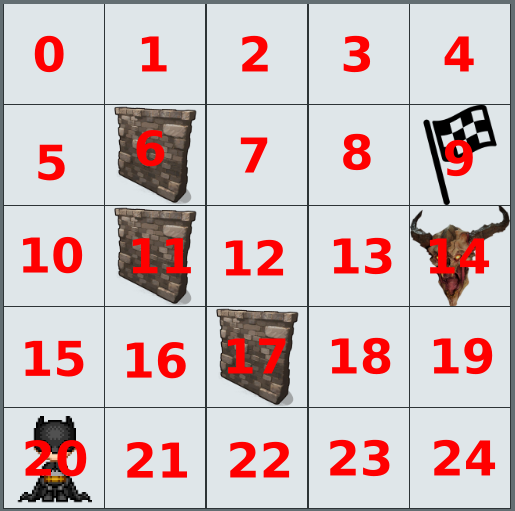
\includegraphics[scale=.4]{img/problemStateEx}}\qquad
    \subcaptionbox{\label{img:problemSolutionEx} Solução}{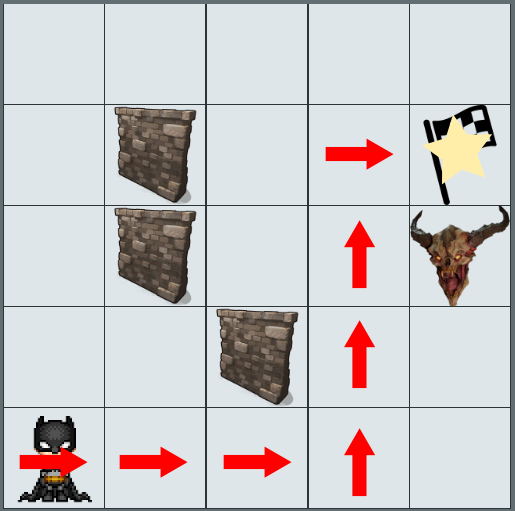
\includegraphics[scale=.4]{img/problemSolutionEx}}
    \vspace{1.5em}
    \legend{\textbf{Fonte:} O Autor}
\label{fig:dag}
\end{figure}

\begin{table}[!htb]
    \centering
    \begin{tabular}{c|c|c|c|c}
            & UP        & DOWN      & LEFT      & RIGHT     \\ \hline
        0   & 2,036     & 3,539     & 2,090     & 5,136     \\
        1   & 3,112     & 2,965     & 4,019     & 6,719     \\
        2   & 4,634     & 4,575     & 4,910     & 9,256     \\
        3   & 7,253     & 13,260    & 6,720     & 13,36     \\
        4   & 11,289    & 20        & 9,250     & 11,322    \\
        5   & 4,147     & 3,144     & 1,406     & 1,004     \\
        6   & 0         & 0         & 0         & 0         \\
        7   & 6,719     & 6,642     & 7,139     & 13,36     \\
        8   & 9,256     & 9,256     & 9,256     & 20        \\
        9   & 0         & 0         & 0         & 0         \\
        10  & 3,548     & 2,898     & 1,090     & 1,130     \\
        11  & 0         & 0         & 0         & 0         \\
        12  & 9,256     & 4,674     & 4,593     &  9,251    \\
        13  & 13,360    & 6,720     & 6,720     & -14,279   \\
        14  & 0         & 0         & 0         & 0         \\
        15  & 3,175     & 3,216     & 0,985     & 3,216     \\
        16  & 1,216     & 3,586     & 2,987     & 1,216     \\
        17  & 0         & 0         & 0         & 0         \\
        18  & 9,256     & 5,153     & 4,720     & 5,153     \\
        19  & -19,999   & 4,076     & 6,720     & 2,966     \\
        20  & 2,988     & 1,216     & 1,216     & 3,586     \\
        21  & 3,216     & 1,586     & 3,216     & 4,185     \\
        22  & 2,185     & 2,185     & 3,586     & 5,153     \\
        23  & 6,720     & 3,153     & 4,185     & 4,185     \\
        24  & 4,956     & 2,184     & 5,153     & 2,183     \\
    \end{tabular}
    \caption{\textit{Q-Table} resultante da execução do experimento.}
    \label{tab:QtableEx}
\end{table}


Estando o personagem inicialmente no estado 20, observando os resultados na \textit{Q-Table}, é
possível traçar o caminho para vitória como o mostrado na Figura \ref{img:problemSolutionEx} que,
notavelmente, é o caminho mais eficiente.

		%--------------------------------------------------------------------------------------
% Este arquivo contém a sua metodologia
%--------------------------------------------------------------------------------------
\chapter{Materiais e Métodos} \label{sec:newModule} %Uma label é como você referencia uma seção no texto com a tag \ref{}

Como já especificado, o trabalho tem como objetivo a investigação de modelos a
serem utilizados no desenvolvimento de um módulo de defesa para o time de
Futebol de Robôs na categoria de simulação 2D, FutVasf2D. O processo de
modelagem de um mundo em um MDP exige a discretização do mesmo de forma que
sejam obtidos um número finito de ações e de estados com os quais o algoritmo de
aprendizado de reforço possa trabalhar, sendo assim, a próxima etapa é definir
como o algoritmo escrito pode ser implementado no time base escolhido
(\textit{WrightEagleBASE}).

\section{Modelagem do Mundo}\label{modelagem}

Os trabalhos apresentados na Seção \ref{trabalhosRelacionados} oferecem várias
possibilidades de como adaptar o ambiente da partida para um problema que se
encaixe às definições de MDP. Algumas das variáveis destacadas por
\citeonline{gabel2008case}, \citeonline{celiberto2007heuristic},
\citeonline{bianchi2010case} e \citeonline{homem2017improving} estão descritos a
seguir:

\begin{itemize}
    \item Posição do jogador;
    \item Posição da bola;
    \item Orientação do corpo do jogador;
    \item Distância entre o jogador e a bola;
    \item Velocidade do jogador;
    \item Distância entre jogador e adversário mais próximo;
    \item Ângulos diversos, como ângulo entre jogador e adversário, ângulo
    formado entre bola, jogador e gol adversário.
\end{itemize}

Segundo \citeonline{Fayyad:1996:DMK:257938.257942}, a Descoberta de Conhecimento
em Base de Dados (do inglês \textit{Knowledge Discovery in Databases} - KDD) é o
processo de identificar padrões válidos, novos, potencialmente uteis, e
inteligível em dados. O KDD é composto de 5 etapas, seleção, pré-processamento,
transformação, mineração de dados e avaliação, como mostrado na Figura
\ref{img:kdd}, junto com cada artefato gerado. Na etapa de pré-processamento são
realizadas manipulação de variáveis pré-existentes e identificações de novas.

\imagem{0.25}{kdd}{Etapas de KDD.}{\cite{Fayyad:1996:DMK:257938.257942}}

A construção de novas variáveis é uma forma sistemática de incorporar
conhecimento em um projeto de KDD. Essas variáveis serão úteis na etapa de
mineração de dados, que no caso de aprendizado por reforço, acontece no momento
do treinamento. Segundo \citeonline{friedman2001elements}, apesar de ser um dos
mais antigos, o processo de construção de novas variáveis é um dos mais
desafiadores. De acordo com \citeonline{witten2016data}, a melhor forma de
construir variáveis é a manual, baseando-se no entendimento do problema e
significado de cada atributo. No geral, essa tarefa depende muito mais do
conhecimento sobre o domínio do que da construção do algoritmo, por tanto, o
conhecimento sobre o domínio é essencial \cite{zhao2009effects}. O uso de
conhecimento de domínio para construção de variáveis aumenta o poder preditivo
do modelo \cite{zhao2009effects}. A estratégia de enriquecimento de dados para
alcançar uma maior capacidade descriminatória é ainda maior em áreas como as de
reconhecimento de som e imagem, de acordo com \citeonline{gao2008wavelet}. As
soluções de melhor performance em competições internacionais utilizaram a
estratégia de construção de novas variáveis a fim de incorporar conhecimento do
domínio, segundo \citeauthoronline{adeodato2009role}
(\citeyear{adeodato2008power}, \citeyear{adeodato2009role}).

Partindo das informações e exemplos obtidos através da revisão bibliográfica,
foram modeladas algumas variações de de formas de representar o mundo. Quatro
componentes são importantes neste processo, os estados que podem ser alcançados
pelo agente, as ações que o mesmo pode tomar, as recompensas e punições a serem
atribuídas para o resultado das ações em cada estado e como será feita a
implementação de todo o modelo no agente. Os 3 primeiros componentes são
cobertos nas subseções abaixo enquanto a implementação é abordada na Seção
\ref{implementacao}.

\subsection{Estados}\label{states}

A definição dos estados é uma etapa certamente crucial e complexa, neste
trabalho foram tomadas duas abordagens. A primeira foi sobre a identificação de
variáveis cujos diferentes possíveis valores formam os estados, a outra se
baseia na identificação de possíveis papéis de função que os agentes podem tomar
no processo de defesa e uma simplificação das possíveis situações que os mesmos
podem estar encaixados.

Especialmente, mas não exclusivamente, na primeira abordagem, é necessário um
cuidado sobre a questão de quais serão os possíveis valores de cada variável,
visto que esta decisão impactará na complexidade e quantidade de estados além
do significado de cada um. Várias das variáveis abordadas a seguir possem
caráter contínuo e uma amplitude de possíveis valores muito grande, por conta
disto foi feita um agrupamento de seus valores em 3 classes através da análise
dos valores assumidos pelas variáveis na execução de várias partidas. As
variáveis identificadas e seus possíveis valores foram as seguintes:

\begin{itemize}
    \item \textbf{Posição do jogador em relação à bola no eixo horizontal}
    ($P_{hj}$), ou seja, se o jogador está mais a direita ou a esquerda da
    bola, esta variável pode assumir valores booleanos onde VERDADEIRO implica
    que o jogador está a esquerda e FALSO a direita;
    \item \textbf{Posição do jogador em relação à bola no eixo vertical}
    ($P_{vj}$), se identifica se o jogador pode ser encontrado mais acima ou
    abaixo da bola, assim como o item passado, os valores assumidos são
    VERDADEIRO para quando o jogador está acima da bola e FALSO quando abaixo,
    esta variável e a anterior são úteis para questão da direção de movimentação
    do jogador;
    \item \textbf{Distância entre o jogador e bola} ($D_{jb}$), mede o
    afastamento do agente em relação à bola, as classes atribuídas para as
    variáveis de distância são as mesmas (PERTO, MÉDIO e LONGE), diferindo
    apenas nos valores atribuídos a cada classe, nesta, os valores para PERTO é
    sempre menor ou igual a 10 (unidade de medida utilizada pelo servidor), para
    MÉDIO os valores são entre 10 e 20 e LONGE engloba todos acima de 20;
    \item \textbf{Distância entre o aliado mais próximo da bola e a bola}
    ($D_{tb}$), aqui os intervalos são menores, podendo assumir PERTO quando o
    valor da distância é menor ou igual a 5, MÉDIO quando entre 5 e 15 e LONGE
    quando acima de 15;
    \item \textbf{O agente é o aliado mais próximo da bola} ($F$), trata-se de
    um valor booleano a fim de identificar se o jogador ``pensante'' é o aliado
    mais próximo à bola;
    \item \textbf{Distância do adversário com posse de bola do gol} ($D_{ag}$),
    mede o afastamento do jogador com posse de bola do gol aliado, aqui os
    valores para PERTO são todos os que forem iguais ou abaixo de 11, MÉDIO
    quando entre 11 e 22 e LONGE quando acima de 33;
    \item \textbf{Compactação} ($\sigma$), consiste numa variável construída a
    partir das distâncias dos jogadores entre si, com foco no adversário com
    posse de bola. Esta variável é importante pois serve como uma maneira de
    reconhecer a dispersão dos jogadores no campo possibilitando o fechamento de
    um ``cerco'' com menos brechas em torno da bola. O cálculo desta variável é
    feito como um desvio padrão com base na distância média entre os jogadores
    aliados e o jogador com posse de bola, como na Equação \ref{eq:desvio}, onde
    $d_i$ é a distância entre o jogador $i$ e o adversário com posse de bola e
    $m$ é a média dessas distâncias, as classes atribuídas a essa variável foram
    ESPARSO (valores acima de 14), COMPACTO (entre 14 e 7) e MUITO COMPACTO
    (abaixo de 7).
\end{itemize}

\begin{equation}
    \sigma=\sqrt{0,1\times \sum{(d_i - m)^2}}
    \label{eq:desvio}
\end{equation}

O estado do modelo descrito, então, passa a ser representado por uma 7-tupla,
($P_{hj}$, $P_{vj}$, $D_{jb}$, $D_{tb}$, $F$, $D_{ag}$, $\sigma$). Como
consequência da quantidade de variáveis e de seus valores, o campo de estados
passa a assumir 648 possibilidades.

Para a segunda abordagem, o campo de estados foi mais simples, baseando-se em
conceitos básicos de defesa no futebol real, foram atribuídos os papéis de
Primeira Defesa, Segunda Defesa e Terceira defesa para o jogador mais próximo da
bola, o segundo mais próximo e o terceiro mais próximo, respectivamente. Além
disso, o valor de compactação já descrito foi reaproveitado para implementar o
conceito de balanceamento no restante do time, resultando na modificação da
Equação \ref{eq:desvio} para a Equação \ref{eq:desvio2} e utilizando o mesmo
conceito de classe anterior, atribuindo-o porém a novos estados ao invés de
valores de um estado único.

\begin{equation}
    \sigma=\sqrt{\frac{\sum{(d_i - m)^2}}{7}}
    \label{eq:desvio2}
\end{equation}

Desta forma essa abordagem resulta num campo de 7 estados que são:

\begin{itemize}
    \item \textbf{Primeira Defesa}, se o agente pensante assume o papel de
    primeira defesa;
    \item \textbf{Primeira Defesa Muito Perto}, se o agente pensante assume o papel de
    primeira defesa e está a uma distância menor oi igual a 5 da bola;
    \item  \textbf{Segunda Defesa}, se o agente tomando a decisão assume o papel
    de segunda defesa;
    \item \textbf{Terceira Defesa}, se agora é assumido o papel de terceira
    defesa;
    \item \textbf{Esparso}, se o jogador não se encaixa nos estados anteriores e
    os jogadores estão muito espalhados no campo;
    \item \textbf{Compacto}, se os jogadores estão menos espalhados;
    \item \textbf{Muito Compacto}, se os jogadores sem papel definido estão
    juntos no campo;
\end{itemize}

Podendo esta modelagem ser considerada muito simples, em outra tentativa foram
atribuídas variações para os jogadores com papéis definidos, resultante no
seguinte campo de 12 estados:

\begin{itemize}
    \item \textbf{Primeira Defesa Muito Perto}, se o agente pensante assume o
    papel de primeira defesa e está a uma distância menor que 5 da bola;
    \item \textbf{Primeira Defesa Perto}, se o agente pensante assume o papel de
    primeira defesa e está a uma distância menor que 6 e maior que 5 da bola;
    \item \textbf{Primeira Defesa Médio}, se o agente pensante assume o papel de
    primeira defesa e está a uma distância menor que 7 e maior que 6 da bola;
    \item \textbf{Primeira Defesa Longe}, se o agente pensante assume o papel de
    primeira defesa e está a uma distância maior que 7 da bola;
    \item \textbf{Primeira Defesa Atrás}, se o agente pensante assume o papel de
    primeira defesa e está atrás da bola;
    \item  \textbf{Segunda Defesa}, se o agente tomando a decisão assume o papel
    de segunda defesa;
    \item  \textbf{Segunda Defesa Com Primeiro Atrás}, se o agente tomando a
    decisão assume o papel de segunda defesa e o agente que assume o papel de
    primeira defesa se encontra atrás da bola;
    \item \textbf{Terceira Defesa}, se agora é assumido o papel de terceira
    defesa;
    \item \textbf{Terceira Defesa Com Segundo Atrás}, se agora é assumido o
    papel de terceira defesa e o jogador que assume o papel de segunda defesa se
    encontra atrás da bola;
    \item \textbf{Esparso}, se o jogador não se encaixa nos estados anteriores e
    os jogadores estão muito espalhados no campo;
    \item \textbf{Compacto}, se os jogadores estão menos espalhados;
    \item \textbf{Muito Compacto}, se os jogadores sem papel definido estão
    juntos no campo;
\end{itemize}

Esses foram os estados utilizados nos experimentos descritos no decorrer deste
trabalho, na subseção seguinte será abordada a questão da escolha de possíveis
ações para os agentes.

\subsection{Ações}\label{actions}

A escolha das ações foi pensando no que pode ser feito, enquanto no papel de
defesa numa partida de futebol, a fim de capturar a bola e impedir o avanço do
time adversário. A implementação original do time base define 3 possíveis ações
para a situação de defesa, mover-se para uma melhor posição, bloquear o avanço
do jogador com posse de bola e marcar adversários para impedir a recepção de
bola. Para este trabalho foram mantidas estas ações com algumas modificações e
adições.

Primeiramente, a ação de se mover foi divida em 5 possíveis ações, mover-se para
cima, para baixo, para esquerda, para direita ou diretamente em direção a bola, desta forma é eliminada a
avaliação original do time base garantido que o aprendizado seja exclusivamente
baseado no algoritmo \textit{Q-Learning}.

Além dessa divisão foi adicionada a ação de interceptação e a possibilidade de
não fazer nada. A ação de interceptação consiste na tentativa de dominar a bola
quando a mesma está ao alcance do agente.

Vale destacar que essas foram as ações levantadas para ser utilizadas, mas isto
não implica que em todos os modelos implementados tenham sido utilizadas todas
as ações.

\subsection{Recompensas}\label{rewards}

As recompensas são partes essenciais do aprendizado por reforço, visto que são
elas as responsáveis por informar ao agente se a ação tomada obteve resultados
positivos ou negativos e o quão positivo ou negativo foi a ação. Esta decisão
não é fácil de ser tomada e por isso foram feitas algumas implementações a fim
de procurar otimizar esses valores.

A primeira tentativa de modelar um bom sistema de recompensas se baseou na
ocorrência dos principais eventos na simulação, gols, bolas jogadas para fora do
campo, captura de bola e passes. Esta modelagem adotou como recompensa para
captura de bola +20, para gols sofridos -20 e para bolas lançadas para fora o
valor +10, visto que implica no sucesso na tentativa de impedir possíveis ações para o
agente adversário, convenção mantida em todas as
modelagens seguintes, e para passe foi atribuído o valor -5 numa tentativa de
impedir o time adversário de se articular.

A segunda implementação aboliu a recompensa de passes e adicionou uma
verificação no avanço e recuo da bola, atribuindo -5 ao avanço da bola, +5 ao
recuo da bola somada à aproximação do agente da captura da bola e +2 ao recuo da
bola sem avanço dos aliados. Esta modelagem se mostrou bastante falha pela
punição excessiva no avanço da bola, visto que ele é uma
característica constante nas situações simuladas, desta forma a última
implementação removeu esta punição e atribuiu recompensa neutra a esta e como
padrão para não identificação de nenhuma das situações anteriores.

\section{Implementação em \textit{WrightEagleBASE}}\label{implementacao}

O último ponto a ser abordado sobre a modelagem está na implementação do
algoritmo, mas para que se possa tratar da implementação realizada, se faz
necessário primeiro entender o funcionamento atual do time base escolhido.

O time base \textit{WrightEagleBASE} conta com um mecanismo modularizado para
tomada de decisões. A sua implementação depende do ``tipo'' de classe
\textit{Behavior} (comportamento), que é constituído por classes mais
especializadas, como comportamento de bloqueio ou de interceptação, e menos
especializadas, como comportamento de defesa ou ataque. As classes menos
especializadas, na implementação original, criam uma forma de hierarquia para
execução das mais especializadas que irão decidir se deve tomar a ação
correspondente a classe ou não. 

Este trabalho foca em 5 dessas classes, \textit{BehaviorDefensePlanner},
\textit{BehaviorFomationPLanner}, \textit{BehaviorBlockPlanner},
\textit{BehaviorMarkPlanner} e \textit{BehaviorInterceptPlanner}, que são
descritas a seguir. O diagrama representado na Figura \ref{img:classDiagram},
mostra como é o diagrama de classes simplificado da implementação original
focando nas classes \textit{Behavior}, mas especificamente na
\textit{BehaviorDefensePlanner}, vale destacar que a classe
\textit{BehaviorPlannerBase} corresponde a uma classe abstrata que é
implementada por todas as demais.

\begin{itemize}
    \item \textbf{\textit{BehaviorDefensePlanner}} decide entre quais
    comportamentos o agente deve decidir quando o time está sem posse de bola e
    em qual ordem, na implementação original apenas define uma ordem de execução
    dos testes de cada possível ação de defesa;
    \item \textbf{\textit{BehaviorFormationPlanner}} coordena a movimentação do
    time, decide quando o agente precisa ser realocado;
    \item \textbf{\textit{BehaviorBlockPlanner}} é responsável por definir
    quando o agente deve tentar bloquear o adversário;
    \item \textbf{\textit{BehaviorMarkPlanner}} decide se há a necessidade de
    determinado agente marcar um adversário;
    \item \textbf{\textit{BehaviorInterceptPlanner}} busca a possibilidade de
    interceptar a bola e se deve tentar realizar tal ação.
\end{itemize}

\imagem{0.5}{classDiagram}{Diagrama de classes simplificado para mecanismo de defesa.}{O Autor}

Um exemplo de como isso é aplicado é dado pela implementação original do
mecanismo de defesa que acontece da seguinte maneira. A classe de defesa define
que a ordem de execução dos planejadores mais específicos é a seguinte:

\begin{enumerate}
    \item \textit{BehaviorFormationPlanner}
    \item \textit{BehaviorBlockPlanner}
    \item \textit{BehaviorMarkPlanner}
\end{enumerate}

Desta forma, o agente primeiro decidirá se precisa se movimentar e para que
local e só em seguida decidirá se precisa realizar um bloqueio e apenas depois
disso, se precisa marcar algum jogador e qual. Desta forma, se garante que o
jogador só se preocupará com bloqueio ou marcação depois de estar na posição
adequada. O fluxograma do algoritmo de decisão das 5 classes,
\textit{BehaviorDefensePlanner}, \textit{BehaviorFormationPlanner},
\textit{BehaviorBlockPlanner}, \textit{BehaviorMarkPlanner}
e \textit{BehaviorInterceptPlanner} podem ser vistas nas
Figuras \ref{img:BehaviorDefense}, \ref{img:BehaviorFormation},
\ref{img:BehaviorBlock}, \ref{img:BehaviorMark} e \ref{img:BehaviorIntercept}, respectivamente.

\imagem{0.8}{BehaviorDefense}{Algoritmo da classe \textit{BehaviorDefensePlanner}}{O Autor}
\imagem{0.5}{BehaviorFormation}{Algoritmo da classe \textit{BehaviorFormationPlanner}}{O Autor}
\imagem{0.8}{BehaviorBlock}{Algoritmo da classe \textit{BehaviorBlockPlanner}}{O Autor}
\imagem{0.8}{BehaviorMark}{Algoritmo da classe \textit{BehaviorMarkPlanner}}{O Autor}
\imagem{0.5}{BehaviorIntercept}{Algoritmo da classe \textit{BehaviorInterceptPlanner}}{O Autor}

Na implementação dos modelos, as classes mais especializadas
(\textit{BehaviorMarkPlanner, BehaviorBlockPlanner, BehaviorFormationPlanner} e
\textit{BehaviorInterceptPlanner}) foram modificadas ou deixaram de ser
utilizadas para melhor se adequar ao processo de tomada de ação proposto.

Desde a primeira implementação do mecanismo de movimento a classe
\textit{BehaviorFormationPlanner} deixou de ser utilizada para dar lugar a
implementação direta do mecanismo de movimentação provido pelo
\textit{framework} do time base. Em uma implementação futura o mesmo foi feito
com as demais classes, mas a principio as classes foram apenas modificadas
removendo as condições que decidiam se a ação deveria ou não ser executada.

Além das classes \textit{Behavior}, são importantes citar duas classes
modificadas no desenvolvimento deste trabalho, são elas \textit{Player} e
\textit{Agent}. A primeira foi utilizada para a implementação da utilização da
\textit{Q-Table} por se tratar de uma etapa esterna aos comportamentos
possibilitando a detecção de eventos que encerra o episódio, como a captura de
defesa, que fazem com que a classe \textit{BehaviorDefensePlanner} não seja
acessada no instante devido. Já a classe \textit{Agent} foi utilizado apenas
como meio de guardar informações sobre o agente a ser compartilhados entre as
classes, visto que esta é a classe responsável pela descrição do agente.

A classe \textit{Player}, portanto, foi tomada com uma certa preocupação devido
ao tempo (medido em ciclos) para se considerar que a ação tomada obteve
resultados. Para tratar desta questão, foi desenvolvido uma fila de ações e seus
respectivos estados para que depois de um determinado número de ciclos pudessem
ser avaliadas, com exceção de estados terminais (como gols, capturas e gols fora
do campo) que quando ocorrem é tomada a primeira ação da fila e em seguida
limpada novamente, tomando assim a ação mais velha que poderia ter causado o
alcance a tal estado. O tamanho da fila foi alterado para tentar chegar ao
melhor valor, assumindo os valores de 2 ciclos, 5 ciclos, 10 ciclos ou 1 ciclo
(ação imediata).

Vale destacar ainda a implementação da \textit{Q-Table} em si, a principio houve
a tentativa de utilizar apenas um arquivo binário com a estrutura de dados de
matriz de \textit{double} para guardar as informações entre todos os agentes
aliados  em campo, porém esta abordagem se mostrou defeituosa por conta da
concorrência do acesso.

A questão é que o time base não faz utilização de \textit{threads}, utilizando
clientes completamente idependentes entre si, em relação a processos, o que
fazia da única forma de controlar o acesso ao arquivo a criação de exclusão de
um arquivo de trava. O problema surgido desta abordagem é a velocidade de
execução dos ciclos que acarretava na verificação por parte de mais de um agente
no momento em que o arquivo de trava ainda não havia sido criado por nenhum
outro, causando sobreposição da tabela sempre que um novo agente terminava de
processar uma ação.

A solução deste problema foi a criação de uma tabela para cada jogador, isto
resolve  o problema da concorrência e trata cada jogador por sua função
especifica no jogo, mas torna o aprendizado potencialmente mais
lento, devido a falta de compartilhamento de experiência. Outra questão desta
abordagem é que obriga a execução do treinamento de todos os jogadores ao mesmo tempo.

\section{Metodologia Experimental}\label{meotodologia}

Os modelos implementados foram treinados com o auxilio da subtarefa HFO,
mostrado na Figura \ref{img:hfo}, que consiste numa especialização do
\textit{RoboCup Simulated Soccer} onde é utilizado apenas metade do campo com
alguns jogadores no ataque e alguns na defesa, foram experimantadas seções de
treinamento utilizando 10 contra 10 jogadores. Com o HFO, é
possível treinar os jogadores para defesa de forma mais objetiva focando apenas
em situações de defesa. Seria possível a execução do treinamento utilizando
partidas completas, no entanto, isso tornaria o treinamento mais lento, já que
seriam encontradas muitas situações diferentes do alvo do trabalho,
resultando em muito tempo na execução de uma partida para poucos episódios
treinados.

\imagem{0.32}{hfo}{HFO}{\url{http://www.cs.utexas.edu/~AustinVilla/sim/halffieldoffense/}}

Devida necessidade de comparar vários modelos e o quão cada um evolue com o
tempo foi utilizado o mecanismo de treinamento para também verificar o
desempenho do modelo em execução. Para este fim foram feitas modificações no
código-fonte com o intuito de contabilizar o número de gols sofridos em
intervalos de 3000 ciclos (metade da quantidade de ciclos de uma partida comum
da categoria) e foram registradas as variações destes resultados para cada
modelo, inclusive o time original sem a técnica empregada.
		\chapter{Resultado e Discussão} \label{sec:results}

Foram identificados os 4 modelos de mundo que demonstraram maior
importância para o estudo, os mesmos estão identificados na Tabela \ref{tab:designs}.

\begin{table}[hbt]
    \centering
    \begin{tabular}{c|c|c|c}
        Modelo & Conjunto de Estados & Conjunto de Recompensas & Tamanho da Fila \\ \hline
        Modelo \customlabel{model:old}{1} & 1 & 1 & 5  \\
        Modelo \customlabel{model:2cycles}{2} & 1 & 2 & 2 \\
        Modelo \customlabel{model:1cycle}{3} & 1 & 2 & 1 \\
        Modelo \customlabel{model:simple}{4} & 2 & 2 & 5 \\ 
    \end{tabular}
    \caption{Modelos de Mundo}
    \label{tab:designs}
\end{table}

Após a execução de grande número de episódios, para treinamento dos modelos
propostos, foram separados em planilhas as quantidades de gols resultantes para
cada bloco de 3000 ciclos para cada um. A partir da execução de 500 blocos
(1.500.000 ciclos) foi feita uma
média geral, uma média dos primeiros 100 registros e uma média de apenas os
últimos 100 registros, levando em conta que se
espera que tenha havido uma melhora na defesa de cada um.

Na Tabela \ref{tab:results} estão listados os modelos de mundo e as médias calculadas e
por fim o valor para comparação do time original. Uma comparação visual é
ilustrada pela Figura \ref{img:averages}.

\definecolor{LightBlue}{rgb}{0.79,0.93,1}

\begin{table}[hbt]
    \centering
    \begin{tabular}{c|c|c|c}
        Modelo & Média Geral & Média dos primeiros 100 blocos & Média dos últimos 100 blocos \\ \hline
        Modelo \ref{model:old} & 44,08 & 44,09 & 44,11  \\
        \rowcolor{LightBlue}
        Modelo \ref{model:2cycles} & 41,48 & 40,21 & 37,82 \\
        \rowcolor{LightBlue}
        Modelo \ref{model:1cycle} & 41,75 & 44,1 & 39,03 \\
        Modelo \ref{model:simple} & 44,69 & 44,4 & 44,77 \\ \hline
        Original &  26,45\\
    \end{tabular}
    \caption{Resultados - Médias de Gols por bloco de 3000 mil ciclos.}
    \label{tab:results}
\end{table}

\imagem{.4}{averages}{Médias finais em comparação ao original}{O Autor}

A observação da Tabela \ref{tab:results} faz com que seja possível perceber que
os modelos de mundo com melhor evolução, ou alguma evolução, são os Modelos
\ref{model:2cycles} e \ref{model:1cycle}. Por conta desta observação foram
realizados um número maior de execuções nos mesmos para que fossem 
traçados gráficos (Figura \ref{img:graph}) cruzando o número de blocos executados no teste e o número de
gols sofridos no último bloco juntamente com a curva de tendência linear formada
por este cruzamento de ambos modelos para que se possa ser feito a visualização
do melhoramento dos mesmos.

\begin{figure}[!htb]
\centering
    \caption{\label{img:graph} Gráficos de Modelos \ref{model:2cycles} e \ref{model:1cycle}}
    \subcaptionbox{\label{img:2cycles} Modelo \ref{model:2cycles}}{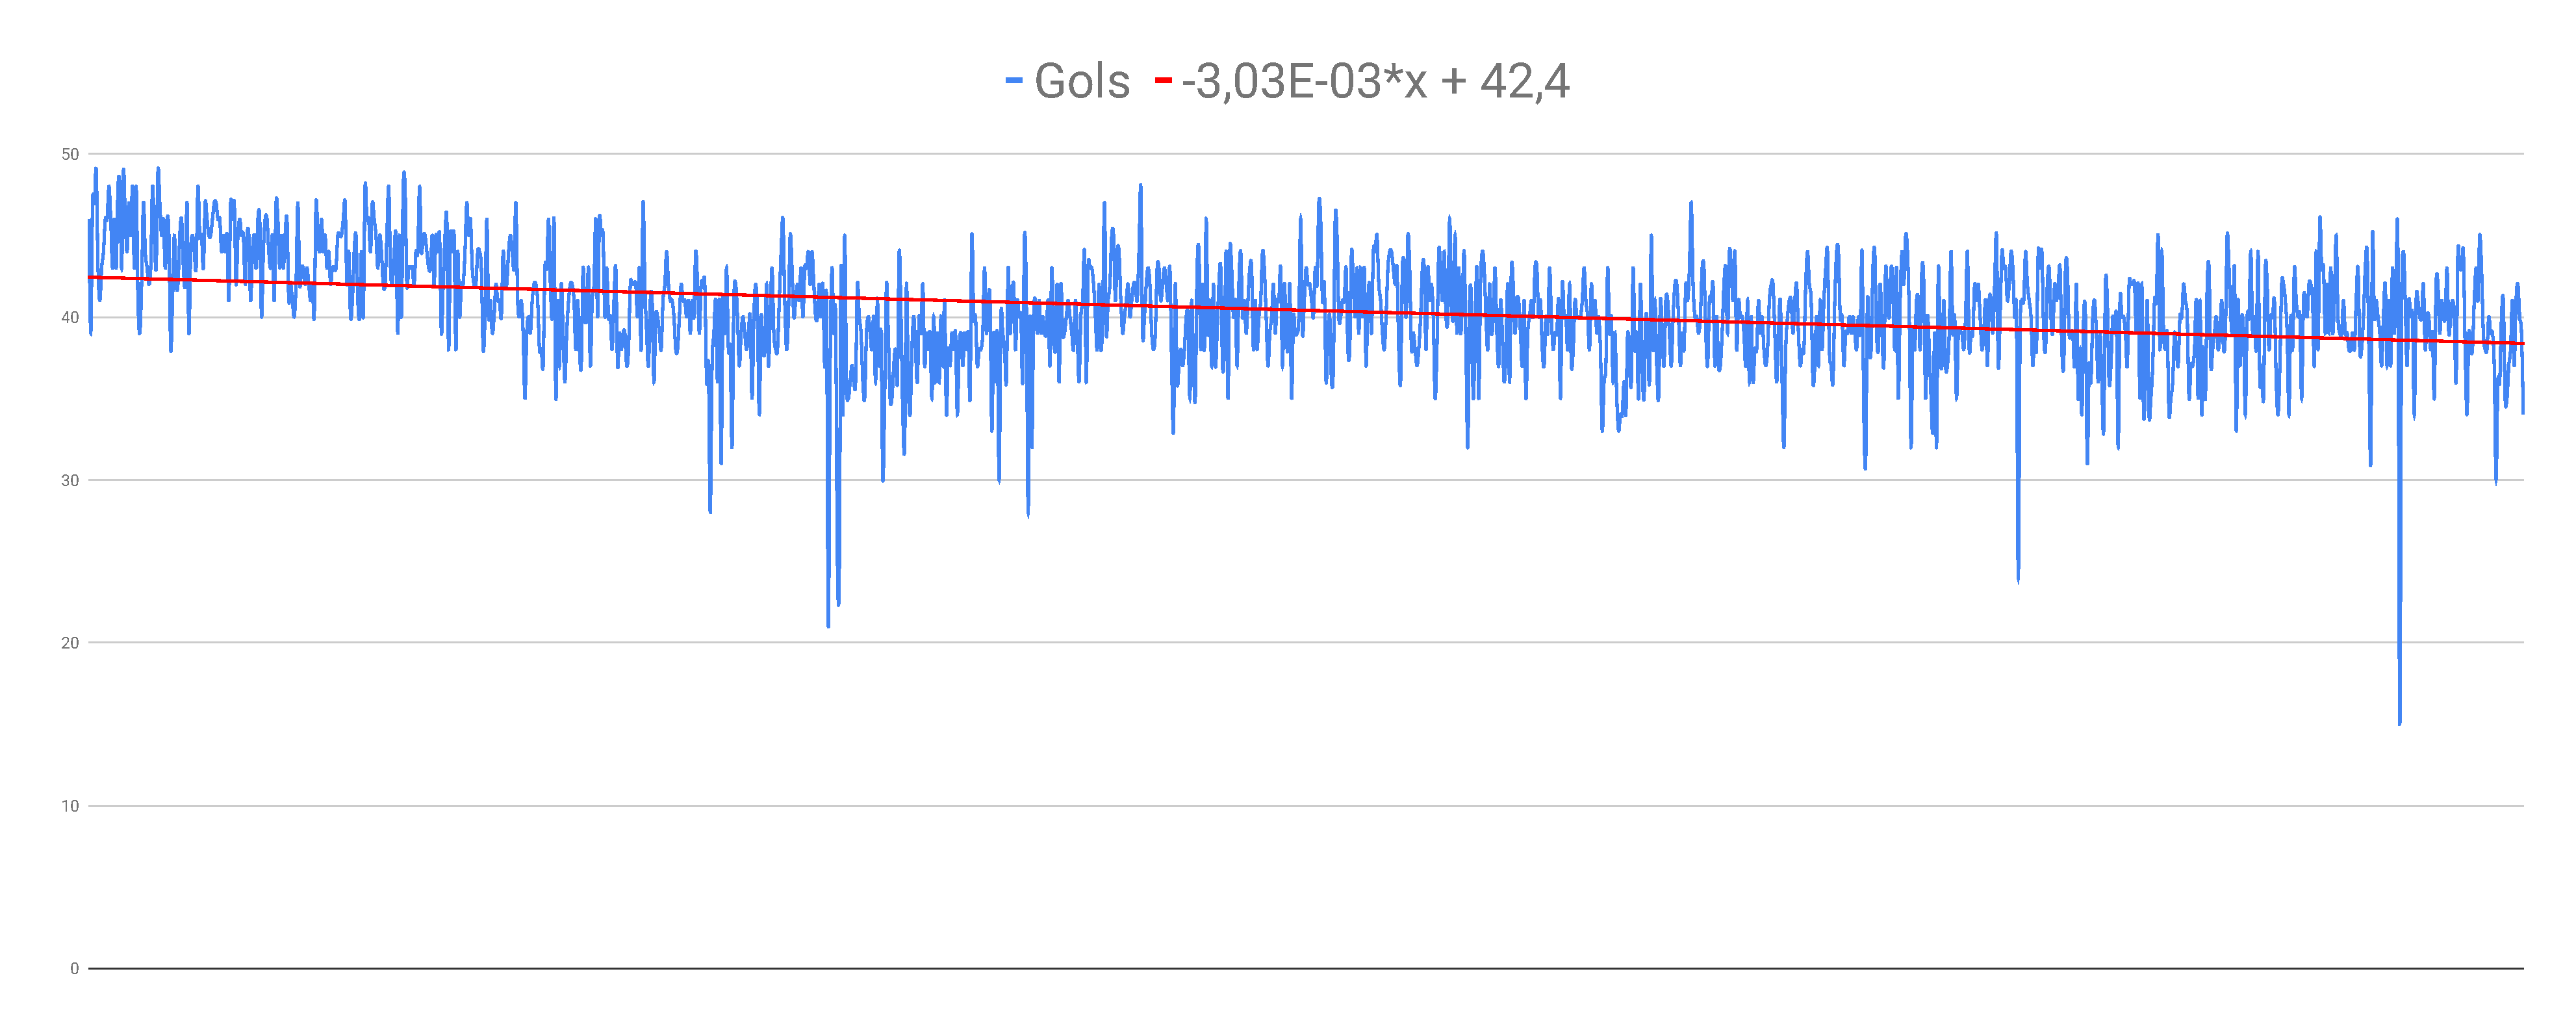
\includegraphics[scale=.235]{img/2cycles}}\qquad
    \subcaptionbox{\label{img:1cycle} Model \ref{model:1cycle}}{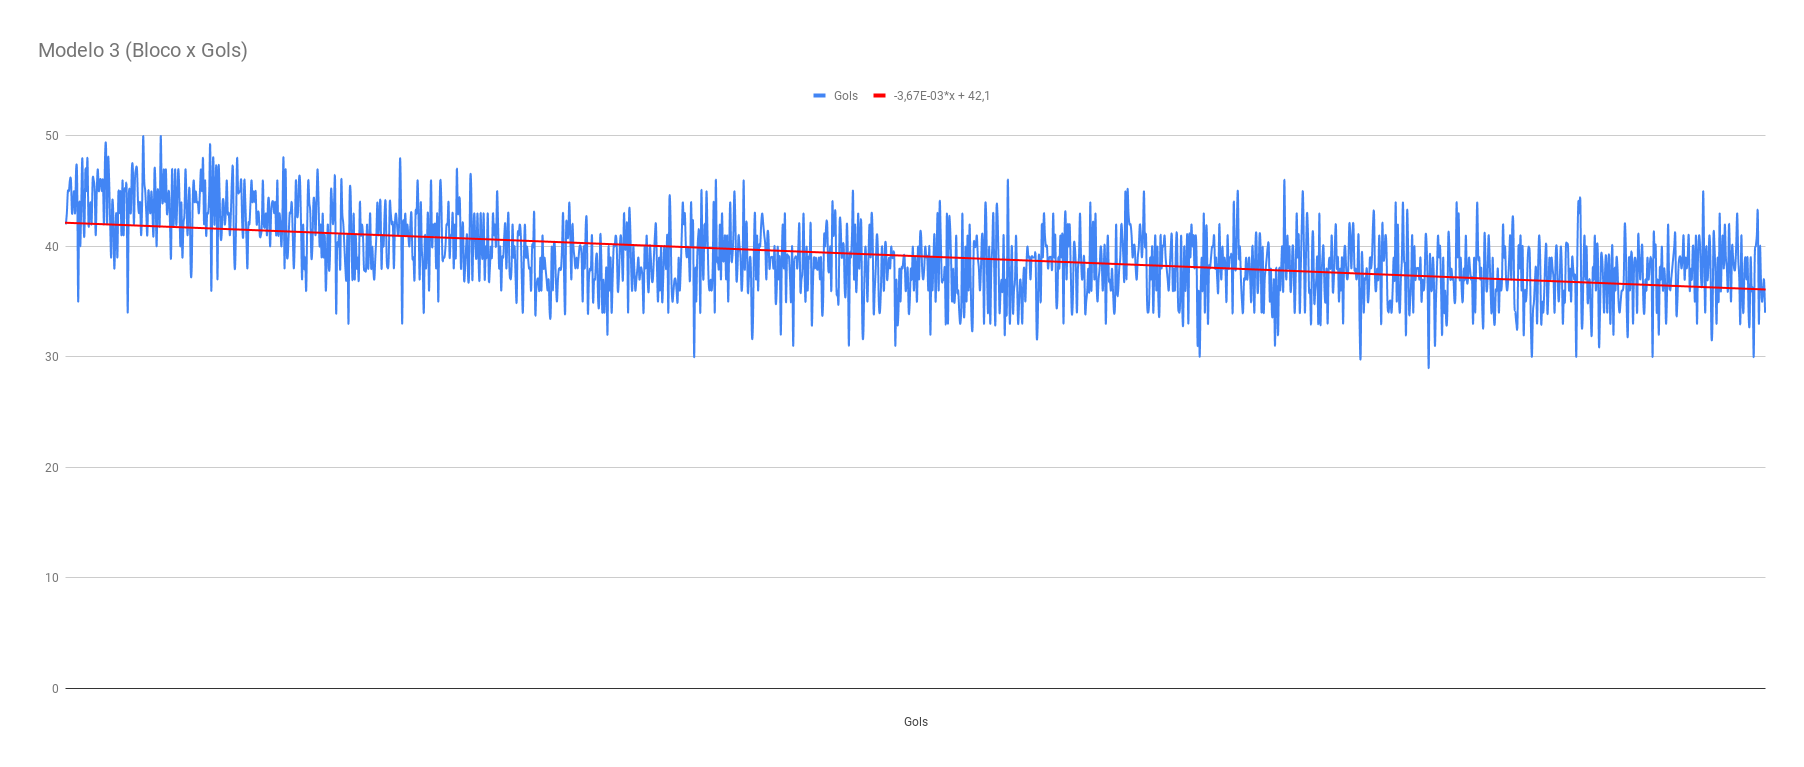
\includegraphics[scale=.25]{img/1cycle}}
    \vspace{1.5em}
    \legend{\textbf{Fonte:} O Autor}
\end{figure}

Os gráficos foram traçados com auxílio da ferramenta de planilhas Google Sheets\footnote{https://docs.google.com/spreadsheets} que
permitiu a captura da equação da curva de tendência traçada. O Modelo
\ref{model:2cycles} é representado pela equação \ref{eq:2cycles} e o Modelo
\ref{model:1cycle} é representado pela Equação \ref{eq:1cycle}, onde $G$
representa a média de gols sofridos por bloco e $b$ o número de blocos executados.

\begin{equation}
    \label{eq:2cycles}
    G=-3,03\times 10^{-3}\times b+42,4
\end{equation}

\begin{equation}
    \label{eq:1cycle}
    G=-3,67\times 10^{-3} \times b+42,1
\end{equation}

É possível observar que os gráficos dos resultados dos Modelos
\ref{model:2cycles} e \ref{model:1cycle} apresentam sinais de evolução na
inteligência dos agentes quanto a tentativa de evitar gols. A análise destes
gráficos, apresentados na Figura \ref{img:graph}, mostra um comportamento
semelhante a ruídos, o que é espererado devido , primeiro, a
característica da simulação que cria ruídos nos sensores dos agentes para que os
mesmos se assemelhem aos sensores falhos dos seres humanos e a característica
aleatória da criação de situações do sistema de treinamento.

Apesar desta observação, como demonstrado na mesma figura e nas Equações
\ref{eq:1cycle} e \ref{eq:2cycles}, que se tratam de regressões lineares dos
resultados encontrados, é possível encontrar um comportamento de melhoria nos
modelos de mundo em questão. Baseando-se em tais equações, é possível extrapolar
um possível valor para o número de blocos a ser executados para que possa ser
superado a média geral do time original, para o Modelo \ref{model:2cycles}, este
número seria de 5265 blocos (mais de 15.000.000 ciclos), já para o Modelo
\ref{model:1cycle} este número seria de 4265 blocos (mais de 12.000.000 ciclos).

É possível, ainda, observar que a tentativa de avaliar a ação tomada após alguns ciclos
de sua execução não apresentou os frutos esperados, pelo contrário, os dois
modelos em destaque foram aqueles com menor número de ações na fila, o que
indica que o melhor momento para colher os resultados de uma ação é o seguinte à
sua execução. Também é
possível observar que a primeira abordagem de estados se mostrou mais
eficiente que a segunda.
		% %--------------------------------------------------------------------------------------
% % Este arquivo contém a sua conclusão
% %--------------------------------------------------------------------------------------
\chapter{Conclusão}\label{sec:conclusion}

Neste capítulo, primeiramente, é feita uma discussão sobre os resultados obtidos
a fim de destacar as contribuições para o futuro do projeto FutVasf2D e o desenvolvimento
de um módulo de defesa para um time de futebol de robôs da liga de simulação 2D.

É possível observar que os gráficos dos resultados dos Modelos
\ref{model:2cycles} e \ref{model:2cycles} apresentam sinais de evolução na
inteligência dos agentes quanto a tentativa de evitar gols. A análise destes
gráficos, apresentados na Figura \ref{img:graph}, mostra um comportamento
semelhante a ruídos, o que é um comportamento espererado devido a, primeiro, a
característica da simulação que cria ruídos nos sensores dos agentes para que o
mesmos se assemelhem aos sensores falhos dos seres humanos e a característica
aleatória da criação de situações do sistema de treinamento.

Apesar desta observação, como demonstrado na mesma figura e nas Equações
\ref{eq:1cycle} e \ref{eq:2cycles}, que se tratam de uma regressão lineas dos
resultados encontrados, é possível encontrar um comportamento de melhoria nos
modelos de mundo em questão. Se baseando em tais equações, é possível extrapolar
um possível valor para o número de blocos a ser executados para que possa ser
superado a média geral do time original, para o Modelo \ref{model:2cycles}, este
número seria de 5265 blocos (mais de 15.000.000 ciclos), já para o Modelo
\ref{model:1cycle} este número seria de 4265 blocos (mais de 12.000.000 ciclos).

Diante dos resultados obtidos através das seções de treinamento, é possível
tomar notas sobre o que pode levar a evolução do projeto e o desenvolvimento de
um módulo de defesa ideal.

Levando em conta todos os modelos de mundo testados e os valores obtidos, é possível
comparar e observar que a tentativa de avaliar a ação tomada após alguns ciclos
de sua execução não apresentou os frutos esperados, pelo contrário, os dois
modelos em destaque foram aqueles com menor número de ações na fila. Também é
possível observar que a primeira abordagem de estados se mostrou mais
eficiente que a segunda.

O resultado deste trabalho serve para apontar novos caminhos a serem tomados
para melhoria de mecanismos de defesa, como o refino dos modelos de mundo aqui indicados
ou a especialização em subtarefas da defesa. Vale a pena focar nos modelos com
melhores resultados deste trabalhos a fim de reproduzi-los e melhora-los.

Uma abordagem interessante a ser tomada para o desenvolvimento de novos modelos
de mundo pode ser a análise do mecanismo já utilizado pelo time original a fim
utilizar o conhecimento já utilizado com o sistema de condicionais para o
melhoramento no campo de aprendizado por reforço.

Também se faz interessante a realização de pesquisas de aplicação do
\textit{Q-Learning} em outros tipos de mecanismos, como no drible ou passe de
bola.

Durante as seções de treinamento foi percebida a necessidade do trabalho no
mecanismo do goleiro, que funciona de forma separada do mecanismo de defesa dos
jogadores comuns. A melhoria do goleiro pode inclusive afetar a forma como os
demais jogadores aprendem, já que com um goleiro mais forte os jogadores teriam
maior liberdade de movimento.

Uma outra possibilidade de pesquisa é a de aplicação de outras técnicas de
aprendizagem de máquina para o mecanismo aqui pesquisado como fim de comparação.

\section{Dificuldades Encontradas}

Durante a execução deste trabalho foram encontrados alguns desafios que
prejudicaram o andamento do mesmo, entre estes pontos estão:

\begin{itemize}
    \item \textbf{Falta de documentação detalhada do time base}, é verdade que o
    time base escolhido (\textit{WrightEagleBASE}) oferece a
    documentação mais completa dentre os principais, mas ainda assim, não é
    fornecido detalhes das funções e classes disponíveis no \textit{framework}
    do mesmo. Isto causa problemas como o desenvolvimento de recursos já
    disponíveis e por vezes menos eficazes;
    \item \textbf{Falta de consistência nos recursos do \textit{framework} do
    time base}, ainda relacionado ao problema anterior, a falta de consistência
    dos recursos causava a utilização de recursos que, embora perfeitamente
    funcionais em certas áreas, não funcionam no local e momento necessários;
    \item \textbf{Concorrência no acesso à \textit{Q-Table}}, este ponto já foi
    abordado na seção \ref{implementacao} e se trata no problema ao acesso para
    leitura e escrita do arquivo relativo à \textit{Q-Table} que fazia com que
    cada agente sobreescrevesse a tabela com seus próprios valores perdendo os
    valores anteriores. Este problema foi contornado através da criação de
    vários arquivos, um para cada agente;
    \item \textbf{Falha na compatibilidade com HFO}. Uma verdade na execução deste trabalho é de que,
    pela sua natureza, foi necessário a execução de treinamentos extensos para
    vários modelos de mundo diferentes. Isto por si só não consistiria em problema, se não
    fosse uma pequena falha na projeção do time base que impedia a plena
    compatibilidade com o HFO. \\
    A falha em questão corresponde a um problema de memória e acesso à ponteiros que
    causa a interrupção dos clientes durante as seções de treinamento, a correção
    desta falha não foi possível por conta da complexidade do código-fonte do time
    base desenvolvido por anos por componentes da equipe \textit{WrightEagle}. Isto
    somado à necessidade de iniciar as seções manualmente, o que impossibilitava a
    escrita de um \textit{script} que reconhecesse a queda dos clientes e o
    executassem novamente, impediu a execução de seções de treinamento longas e
    initerruptas;
    \item \textbf{Quantidade de recursos exigidos}. Outro prolema relacionado à execução dos treinamentos é quantidade de recursos
    utilizadas pelo treinamento, já que o HFO utiliza o máximo que consegue dos
    recursos para executar ciclos rápidos agilizando o treinamento. O consumo em
    questão impossibilitou a execução de treinamento de mais modelos de mundo
    simultaneamente.
\end{itemize}

Tudo isso somado a quantidade de variáveis que precisavam ser testadas para que
se pudesse obter uma otimização do modelo e da implementação do mesmo impediu
exploração maior nas possibilidades levantadas.

	\postextual
		\bibliography{tex/references}
		\begin{apendicesenv}
    \chapter{Códigos-Fonte}
    \sourcecodenolist{\textit{Player} - Avaliação de Ação e Atualização de \textit{Q-Table}}{alg}{cpp}{Player.cpp}

    \sourcecodenolist{\textit{BehaviorDefensePlanner} - Identificação de Estado e Escolha de Ação Para Model \ref{model:simple} (Mais Simples)}{alg}{cpp}{BehaviorDefense.cpp}
\end{apendicesenv}

\end{document}
